% -*- root: projekt.tex -*-

\chapter{Úvod}

Rozvoj informačních technologií postupuje vpřed rychlým tempem a objevují se nové a efektivnější algoritmy. Přesto existují problémy, které neumíme řešit běžným \uv{inženýrským} přístupem, protože zatím nebyl objeven vhodný teoretický popis. I~pokud takový popis existuje, zahrnuje pouze podmnožinu všech možných reprezentací řešení. Prohledáváním v~prostoru všech možných kombinací dostupných výpočetních prvků pak můžeme nalézt řešení, kterých nelze dosáhnout konvenčními metodami, ale mohou mít některé velmi výhodné vlastnosti. I~když je dnes běžně dostupný dříve nepředstavitelný výpočetní výkon, je mnohdy nemožné prohledat celý prohledávací prostor a vybrat nejlepší řešení. Proto se používají metody, které se snaží usměrňovat prohledávání správným směrem a zároveň prohledávaný prostor co nejvíce zmenšit, to vše aniž by utrpěla kvalita nalezeného řešení.

Mnohé metody umělé inteligence se inspirují v~přírodě, například neuronové sítě, mravenčí kolonie, výpočty simulující rojení hmyzu nebo evoluční algoritmy, které mají svůj základ v~Darwinově teorii o~vzniku druhů. Evoluční algoritmy se ukazují jako výhodné pro různé optimalizační problémy, ale také lze pomocí genetického programování automaticky tvořit počítačové programy, elektrické obvody, optické systémy a dokonce i umělecká díla.

Jednou z~úspěšných aplikací genetického programování je automatizovaná tvorba obrazových filtrů. Ty umožňují zrekonstruovat obrázky poškozené při přenosu dat nebo kvůli nefunkčním bodům ve snímači fotoaparátu či kamery. Často jsou součástí předzpracování dat u~úloh zpracovávajících obraz a na jejich kvalitě závisí úspěšnost celého algoritmu. Také jsou významné v~kosmonautice, kde je obtížné zamezit chybám při přenosu fotografií na Zemi nebo dokonce opravit či vyměnit kameru umístěnou na vesmírné sondě.

Tato práce se zabývá návrhem programu, který bude schopen tvořit obrazové filtry pomocí koevolučního algoritmu. Vedle obrazových filtrů se vyvíjí i populace tzv. prediktorů fitness, které slouží k~urychlení výpočtu kvality každého vytvořeného filtru. Protože výběr vhodné velikosti prediktorů není triviální a někdy je nutné ke stanovení správné hodnoty provést velké množství experimentů, je nově do algoritmu zahrnuto souběžné učení, jehož cílem je adaptovat velikost prediktorů na aktuální průběh evoluce filtrů.

Tento semestrální projekt je strukturován následovně: Kapitola~\ref{chEA} se zabývá evolučními algoritmy. Nejprve jsou představeny obecné principy evolučních algoritmů (v~části~\ref{secEAGeneral}), genetický algoritmus~\ref{secGA} a kartézské genetické programování~\ref{secCGP}. Následuje popis návrhu obrazových filtrů~\ref{secIF}. Předposlední část~\ref{secCoev} je věnována koevolučním algoritmům, především ve spojitosti s~kartézským genetickým programováním, a závěrečná část~\ref{secColearning} se zabývá souběžným učením, Baldwinovým efektem a plasticitou fitness. Kapitola~\ref{chDesign} se zabývá návrhem řešení tvorby obrazových filtrů s~použitím koevolučního algoritmu se souběžným učením, které bude implementováno v~diplomové práci.

\chapter{Evoluční algoritmy}
\label{chEA}

První evoluční algoritmy se v~literatuře objevují od 50. let 20. století. Postupně a nezávisle na sobě vzniklo několik podobných metod (například evoluční strategie, evoluční programování nebo genetické algoritmy), které se v~různých obměnách používají i dnes. Až s~rozšířením spolupráce mezi těmito nezávislými výzkumnými týmy v~90. letech vznikl pojem \uv{evoluční algoritmus} \cite{Modra}.

\section{Základní principy evolučních algoritmů}
\label{secEAGeneral}

Evoluční algoritmy jsou stoachastické optimalizační metody inspirované přírodou, konkrétně Darwinovou teorií evoluce. Ačkoliv pojmy používané v~evolučních algoritmech vycházejí z~biologie, jejich význam není vždy přesně stejný. Mezi základní pojmy patří:

\begin{itemize}
    \item\emph{Gen} je základním stavebním blokem kandidátního řešení, je omezen předem danou abecedou (binární čísla, písmena apod.),
    \item\emph{Alela} je konkrétní varianta genu,
    \item\emph{Chromozom} nebo \emph{jedinec} reprezentuje jedno řešení ve stavovém prostoru,
    \item\emph{Genotyp} je posloupnost genů kódující řešení,
    \item\emph{Fenotyp} je kandidátní řešení odvozené z~genotypu,
    \item\emph{Populace} je konečná množina kandidátních řešení,
    \item\emph{Fitness} udává \uv{kvalitu} jedince s~ohledem na řešený problém,
    \item\emph{Fitness funkce} přiřazuje každému jedinci právě jedno reálné číslo -- hodnotu fitness,
    \item\emph{Diverzita} udává rozmanitost populace, tj. nakolik se od sebe chromozomy v~populaci navzájem liší.
    %\item\emph{Rodiče} jsou podmnožina populace, ze které budou vytvořeni \emph{potomci}.
\end{itemize}

Typickým rysem evolučních algoritmů je to, že pracují s~populací několika kandidátních řešení, od kterých odvozují nová řešení pomocí speciálních biologií inspirovaných operátorů. Jednoduchý evoluční algoritmus znázorňuje schéma~\ref{obrEA} a lze zapsat takto:

\begin{enumerate}
    \item Náhodně vygeneruj populaci o~dané velikosti.
    \item Opakuj dokud není splněna ukončovací podmínka:
    \begin{enumerate}
        \item urči fitness jedinců v~populaci,
        \item z~populace vyber rodiče a vytvoř potomky,
        \item některé jedince v~populaci nahraď potomky.
    \end{enumerate}
    \item Výsledkem je jedinec s~nejvyšší fitness (nejlepší nalezené řešení problému).
\end{enumerate}

\begin{figure}[htb]
    \centering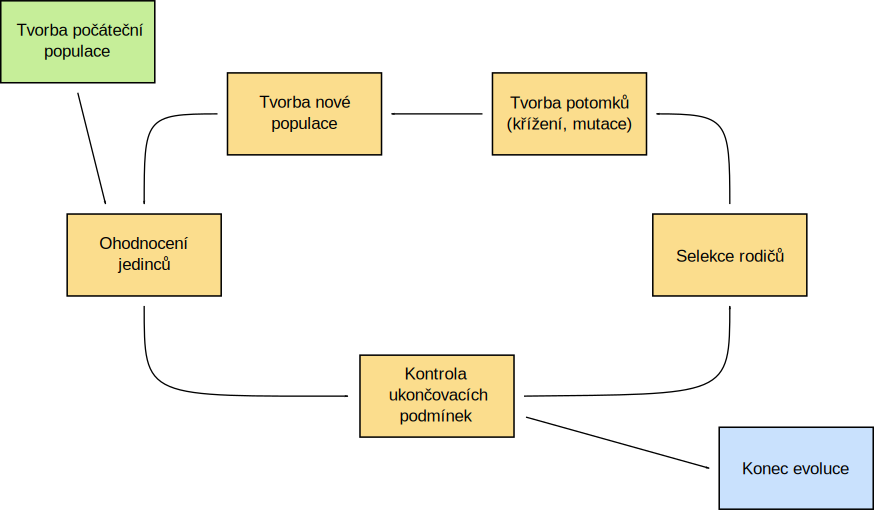
\includegraphics[width=0.85\textwidth]{fig/ea.pdf}
    \caption{Schéma evolučního algoritmu.}
    \label{obrEA}
\end{figure}

Nevýhodou evolučních algoritmů je velké množství parametrů a podproblémů. Před samotným výpočtem pomocí evolučního algoritmu je třeba si položit například tyto otázky:

\begin{itemize}
    \item Jak se budou kódovat kandidátní řešení do genotypu?
    \item Kolik jedinců má být v~populaci?
    \item Jak se budou vybírat rodiče nové populace?
    \item Jak se budou tvořit potomci?
    \item Kolik jedinců v~populaci má být nahrazeno potomky?
\end{itemize}

Je třeba brát v~potaz i stochastickou povahu evolučních algoritmů, z~čehož plyne, že pro porovnání různých algoritmů (nebo různých hodnot parametrů) je potřeba statisticky vyhodnotit větší množství běhů \cite{HandbookEA, Modra}.


\section{Genetický algoritmus}
\label{secGA}

Genetický algoritmus byl vytvořen Johnem Hollandem v~sedmdesátých letech. Samotný termín \uv{genetický algoritmus} se začal běžně používat až po publikaci dizertační práce Kena De Jonga v~roce 1975. Do širšího povědomí se dostává v~půlce osmdesátých let, kdy se ukázalo, že jej lze použít k~řešení řady obtížných úloh.

%Existují i hybridní genetické algoritmy, ve kterých se uplatňuje lokální prohledávání.

Schéma genetického algoritmu odpovídá obecnému evolučnímu algoritmu. Počáteční populace je vytvořena náhodně. V~každé iteraci se populace ohodnotí (určí se fitness jedinců) a podle zvoleného selekčního algoritmu se vyberou rodiče, ze kterých jsou pomocí operátorů křížení a mutace vytvořeni potomci. Kromě potomků je možné v~nové populaci zachovat i několik jedinců z~původní populace (s~případnou mutací). Pokud se používá \emph{elitismus}, je nejlepší jedinec vždy součástí nové populace \cite{Modra, HandbookGA}.


\subsection{Reprezentace řešení}

Genotyp v~genetickém algoritmu je často jednoduchá datová struktura, jako je vektor bitů nebo čísel konstantní délky. V~případně binárního chromozomu může být vhodné použít Grayovo kódování, ve kterém se dvě po sobě jdoucí hodnoty liší vždy pouze jedním bitem. To pomáhá překonat tzv. Hammingovu bariéru, kdy malá změna v~genotypu způsobí velkou změnu ve fenotypu a naopak. Například ve fenotypu je mezi čísly 15 a 16 malý rozdíl, ale v~binárním genotypu se liší o~5 bitů \cite{HandbookGA}.


\subsection{Selekce rodičů}

Volbu $K$ rodičů z~populace lze provést několika způsoby. Nejjednodušší je prosté seřazení jedinců podle jejich fitness, rodiči se pak stává $K$ jedinců s~nejvyšší fitness. O~trochu složitější je ruletová a turnajová selekce, které znázorňuje obrázek~\ref{obrSelekce}.

U~\emph{ruletové selekce} je pravděpodobnost, že se konkrétní jedinec stane rodičem, přímo úměrná jeho fitness:

\begin{equation}
p_i = \frac{f_i}{\sum_{j=1}^N{f_j}}
\end{equation}

\noindent{}Lze si to představit jako ruletu, kde každá výseč odpovídá jednomu jedinci a čím vyšší má jedinec fitness, tím je příslušná výseč větší. Nevýhodou je, že pokud má jeden nebo více jedinců výrazně vyšší fitness než zbytek, stávají se tito jedinci téměř vždy rodiči a zmenšuje se diverzita populace. Jedním ze způsobů, jak lze tento problém řešit je, že se jedinci seřadí podle velikosti fitness a pravděpodobnost výběru je úměrná pořadí jedince a ne jeho fitness.

Jiným přístupem k~výběru rodičů je \emph{turnajová selekce}. Do turnajového kola jsou náhodně vybráni dva nebo více jedinců. Vítězem kola se stává jedinec s~nejvyšší fitness a ten se stává rodičem. Turnaj se opakuje tolikrát, kolik rodičů je potřeba zvolit. Může se stát, že mezi rodiči se bude některý jedinec opakovat \cite{Modra}.


\begin{figure}[hbt]
    \centering
    \subfigure[Ruleta podle fitness]{
        \label{obrSelekceR1}
        \centering
            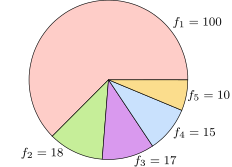
\includegraphics[width=0.27\textwidth]{fig/ruleta1b.pdf}
    }
    \hfill
    \subfigure[Ruleta podle pořadí]{
        \label{obrSelekceR2}
        \centering
            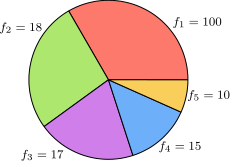
\includegraphics[width=0.27\textwidth]{fig/ruleta2b.pdf}
    }
    \hfill
    \subfigure[Turnaj]{
        \label{obrSelekceT}
        \centering
            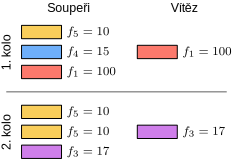
\includegraphics[width=0.27\textwidth]{fig/turnajb.pdf}
    }
    \caption{Mechanismy selekce v~genetickém algoritmu.}
    \label{obrSelekce}
\end{figure}



\subsection{Křížení}

Křížení je považováno za hlavní operátor genetického algoritmu. Během něj je vytvořen nový jedinec jako kombinace genů dvou nebo více chromozomů. Obrázek~\ref{obrKrizeni} znázorňuje tři základní mechanismy: jednobodové, vícebodové a uniformní křížení. U~\emph{jednobodového křížení} je náhodně zvolen bod, ve kterém se chromozomy rozdělí a geny za tímto bodem si mezi sebou vymění. U~\emph{vícebodového křížení} je těchto bodů několik. V~případě \emph{uniformního křížení} se rozhoduje, zda dojde k~prohození nebo ne, u~každého genu zvlášť \cite{Modra}.

\begin{figure}[htb]
    \centering
    \subfigure[Jednobodové]{
        \centering
            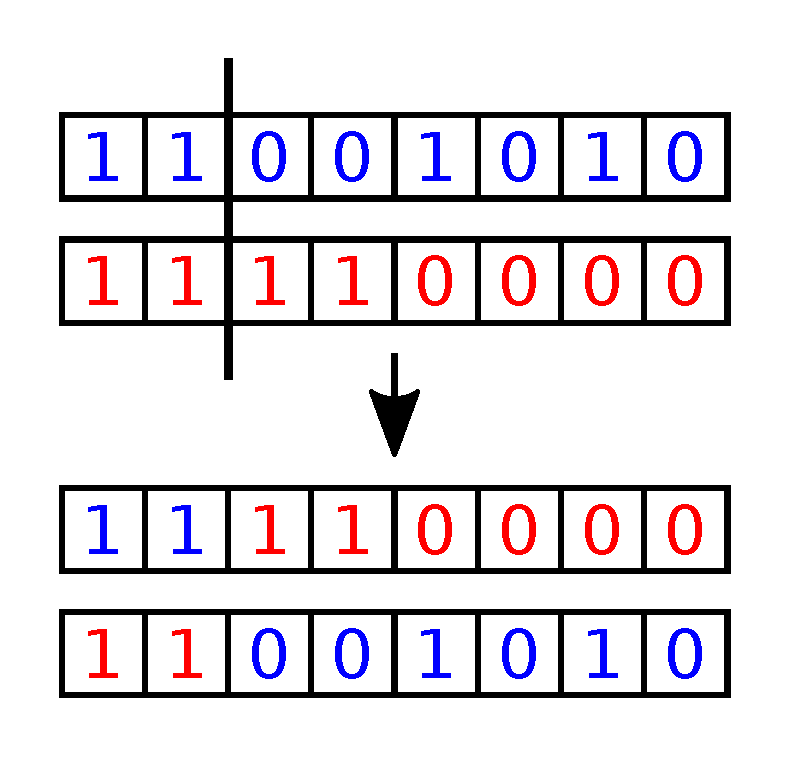
\includegraphics[width=0.2\textwidth]{fig/crossover1.pdf}
    }
    \hskip1.5cm
    \subfigure[Vícebodové]{
        \centering
            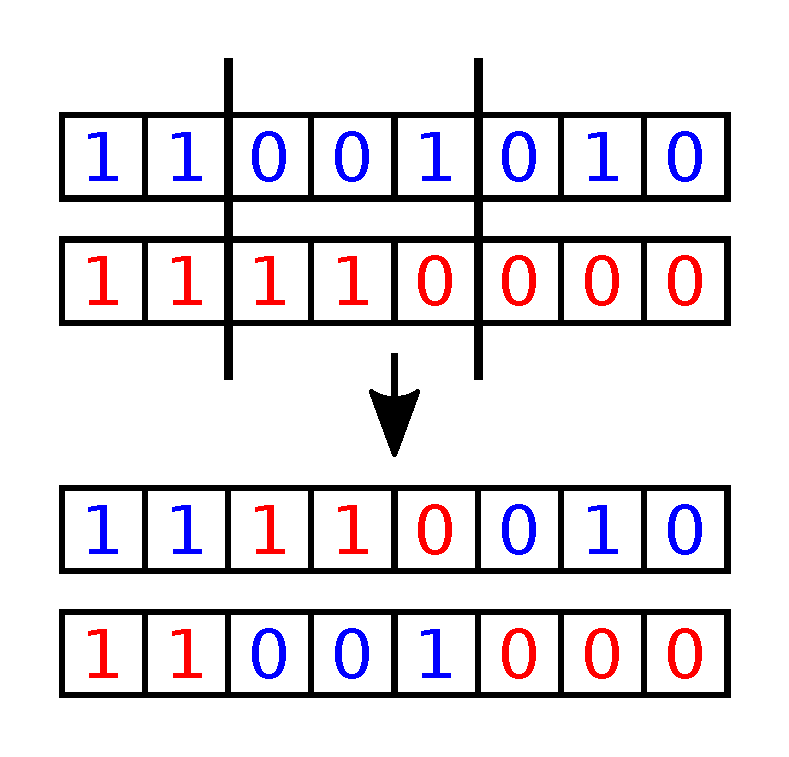
\includegraphics[width=0.2\textwidth]{fig/crossover2.pdf}
        }
    \hskip1.5cm
    \subfigure[Uniformní]{
        \centering
            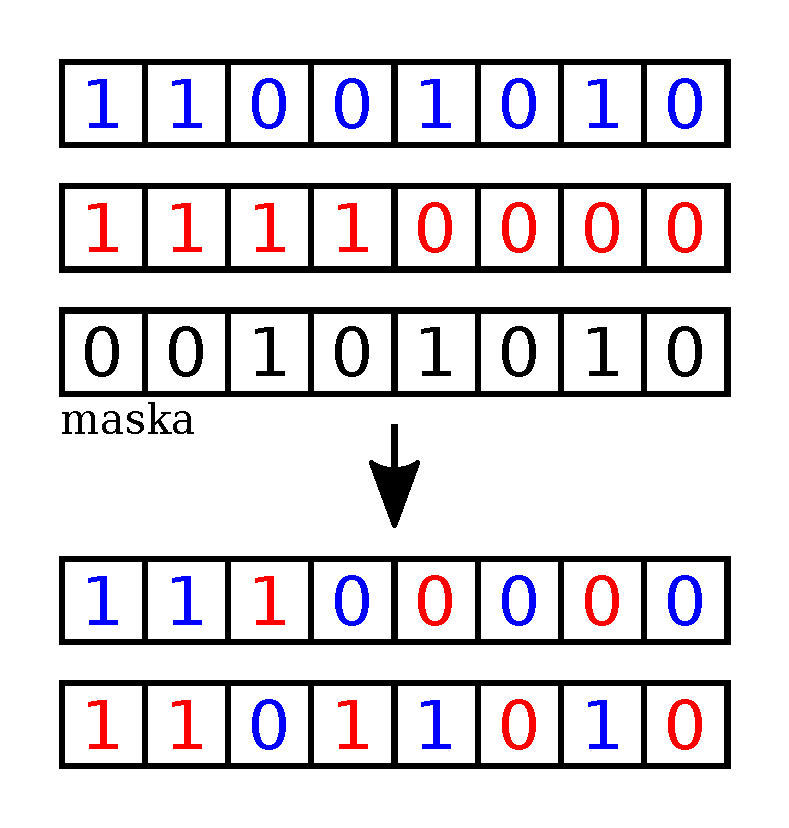
\includegraphics[width=0.2\textwidth]{fig/crossoverU.pdf}
        }
    \caption{Tři základní mechanismy křížení v~genetickém algoritmu.}
    \label{obrKrizeni}
\end{figure}


\subsection{Mutace}

Mutace je malá změna genotypu, která se s~malou pravděpodobností provádí u~potomků vzniklých křížením. V~případě binárně kódovaného chromozomu mutace spočívá v~překlopení několika náhodně zvolených bitů. U~celočíselného kódování je hodnota genu nahrazena náhodným číslem. Existují také speciální mutační operátory pro reálná čísla nebo pro permutačně kódované chromozomy. Pokud je z~povahy problému hodnota genu omezená výčtem nebo intervalem, je vhodné, aby výsledkem mutace nebyla nepřípustná hodnota, aby nevznikala neplatná řešení \cite{Modra}.

\section{Kartézské genetické programování}
\label{secCGP}

Další variantu evolučního algoritmu, genetické programování, představil koncem 80.~let 20.~století John Koza. Umožňuje automatizovanou tvorbu celých programů, kdy neřeší jak má program pracovat, pouze co má být jeho výstupem. John Koza pracoval s~jazykem LISP, pro který je vhodná reprezentace programu pomocí stromů. Existují ale i jiné způsoby kódování programů do chromozomu, například ve formě kartézských programů. Kartézské genetické programování (CGP) představil Julian Miller koncem devadesátých let \cite{Miller2000}.

V~CGP se programy kódují jako orientované acyklické grafy, reprezentované dvourozměrnou kartézskou mřížkou výpočetních uzlů (funkčních bloků) o~předem daných rozměrech. Příklad kartézského programu je zobrazen na obrázku~\ref{obrCGP}. Počet primárních vstupů a výstupů je fixní. Každý výpočetní uzel vykonává nějakou funkci z~předem daného seznamu. Ten je vhodné přizpůsobit řešené úloze, například pro tvorbu logických obvodů to mohou být dostupná logická hradla, pro symbolickou regresi to mohou být aritmetické operace apod. Vstupy funkčních bloků jsou napojeny buď na některý z~primárních vstupů, nebo na výstup uzlu umístěného v~některém sloupci nalevo. O~kolik sloupců doleva je možné uzly propojovat určuje parametr $l$-back. Pokud je roven jedné, je možné propojovat pouze uzly ze sousedních sloupců, pokud je $l$-back roven počtu sloupců, lze uzly propojovat libovolně. Zpětné vazby a cykly nejsou v~CGP povoleny.

\begin{figure}[htb]
    \centering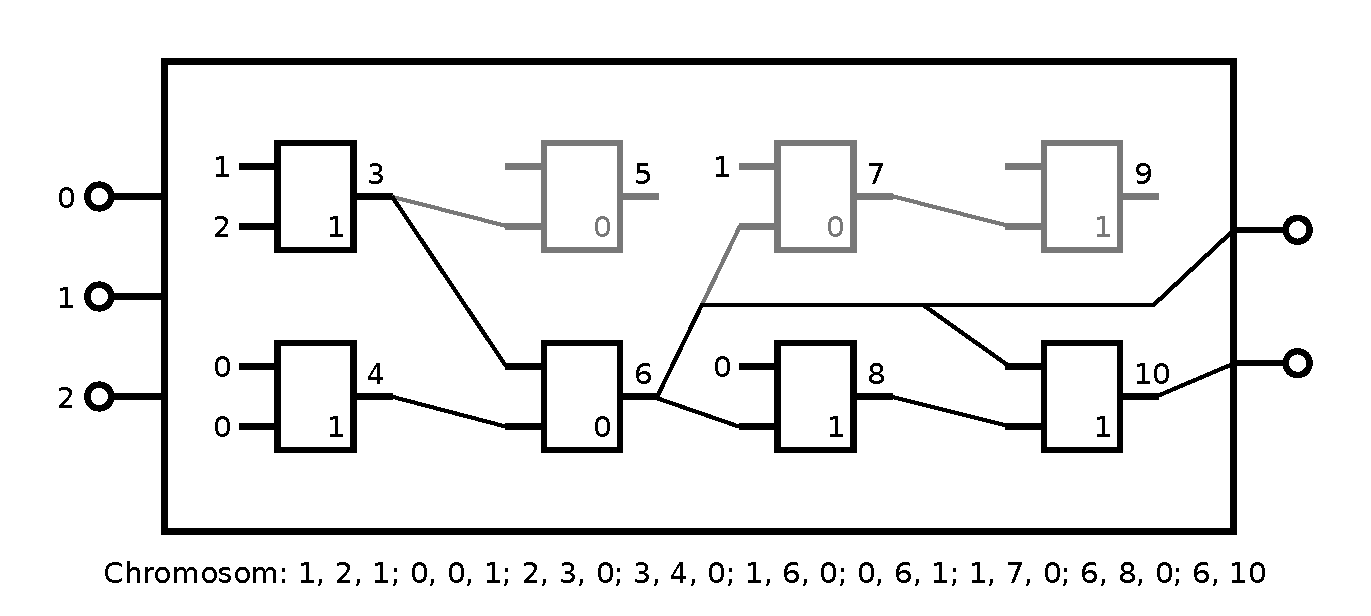
\includegraphics[width=0.6\textwidth]{fig/cgp.pdf} \\
    {\scriptsize{}Chromozom: \{1, 2, A; 0, 0, A; 2, 3, B; 3, 4, B; 1, 6, B; 0, 6, A; 1, 7, B; 6, 8, B; 6, 10\}}
    \caption{Program v~kartézském genetickém programování. Uzly 5, 7 a 9 jsou neaktivní.}
    \label{obrCGP}
\end{figure}

Chromozom je posloupnost celých čísel konstantní délky, jednotlivé geny určují funkci výpočetních uzlů a jejich propojení. Na konci chromozomu je pro každý primární výstup jeden gen obsahující číslo uzlu, jehož výstup má být použit. Velikost fenotypu je variabilní, ale nikdy nepřesáhne velikost genotypu. Je to proto, že ne všechny funkční bloky jsou přímo či nepřímo napojeny na primární výstupy programu -- hovoříme o~\emph{neaktivních blocích}.

Výhodou kartézského genetického programování je omezený stavový prostor, nehrozí, že by délka programu během evoluce rostla nad únosnou mez, tak jako u~stromové reprezentace. Prohledávací prostor lze dále omezovat parametrem $l$-back a omezením množiny dostupných funkcí \cite{ZelenaCGP, Modra, HandbookGP}.

\subsection{Průběh evoluce}
\label{secCGPEvo}

Schéma evoluce opět odpovídá obecnému evolučnímu algoritmu. Počáteční populace je vygenerována náhodně. Oproti genetickému algoritmu se u~kartézského genetického programování většinou nepoužívá křížení, protože jeho přínos pro konvergenci řešení není velký. Po ohodnocení všech jedinců je nejlepší z~nich určen rodičem. Ostatní jedinci jsou nahrazeni potomky -- náhodnými mutacemi rodiče. Tento způsob tvorby nových generací se označuje jako evoluční strategie $(1 + \lambda)$ \cite{Modra}.

\subsection{Mutace}

Mutace mění náhodně hodnotu některých genů jedince. Jejich počet se běžně volí jako procento z~celkového počtu genů, označované jako \emph{míra mutace}. Geny nelze nahrazovat libovolnými hodnotami, je třeba brát ohled na parametr $l$-back, počet primárních vstupů a počet dostupných funkcí pro výpočetní uzly:

\begin{itemize}
    \item U~genu kódujících funkci, je náhodně vygenerován index funkce ze seznamu dostupných funkcí.
    \item U~genu kódujících vstup funkčního bloku jsou povolenými hodnotami:
        \begin{itemize}
            \item číslo primárního vstupu programu,
            \item číslo některého uzlu ze sloupců nalevo, s~ohledem na parametr $l$-back.
        \end{itemize}
    \item U~genu kódujících primární výstup je náhodně vybráno číslo některého výpočetního uzlu nebo primárního vstupu.
\end{itemize}

Ne každá mutace vede na změnu fenotypu -- například může dojít ke změně funkce neaktivního bloku nebo propojení mezi neaktivními bloky. Ukazuje se ale, že i tyto tzv. \emph{neutrální mutace} jsou prospěšné pro konvergenci algoritmu. Proto pokud je v~populaci několik nejlepších jedinců se stejnou hodnotou fitness, je vhodné vybírat jako rodiče toho, který nebyl rodičem v~předchozí generaci, tj. chromozom, který vznikl neutrální mutací. V~opačném případě, kdy se rodičem může stát pouze jedinec s~vyšší hodnotou fitness, evoluce nachází méně kvalitní programy.

Ačkoliv mutace mění pouze malý počet genů a v~genetických algoritmech slouží spíše jako doplňkový operátor, v~případě CGP může malá mutace vést na velkou změnu fenotypu. Například po změně pouze jednoho propojení funkčních bloků se může funkce programu zásadně změnit, protože se najednou stane aktivními větší množství funkčních bloků. Mutace tak v~CGP slouží i jako extenzivní operátor \cite{ZelenaCGP, Modra}.

\subsection{Výpočet fitness}
\label{secFitnessCalc}

Genetické programování umožňuje automatizovaně vytvářet programy s~požadovaným chováním. Chování -- požadované odezvy programu na zadané vstupy -- je definováno v~tzv. \emph{trénovací množině}. Každý prvek této množiny reprezentuje jeden \emph{případ fitness}. Například pokud je cílem nalézt program aproximující polynom $x^4 + x^3 + x^2 +x$ nad množinou přirozených čísel menších než deset, je každé z~těchto čísel jedním případem fitness. V~případě programu $x^2 + 1$ je hodnota $2^2 + 1 = 5$ odezva programu pro případ fitness $2$. Fitness kandidátního řešení je pak určena jako součet odchylek požadovaného a skutečného výstupu programu pro všechny případy fitness z~trénovací množiny.

U~složitějších problémů může být takových případů fitness velmi mnoho. Protože výpočet fitness je časově nejnáročnější částí evoluce, je vhodné do trénovací množiny zahrnout pouze část případů fitness a urychlit tak výpočet. Na druhou stranu je třeba velikost množiny a používané případy fitness zvolit tak, aby byly i pro kombinace vstupů neobsažené v~trénovací množině byly výstupy programu v~souladu s~požadovaným chováním.

%Každý prvek této množiny tvoří jeden \emph{případ fitness}.

%Případy fitness typicky tvoří malý vzorek stavového prostoru. Výběr tohoto vzorku a jeho velikosti zásadně ovlivňuje kvalitu nalezených programů a dobu běhu evoluce. Menší vzorek vede na

%Genetické programování umožňuje automatizovaně vytvářet programy s požadovaným chováním. Jednotlivé prvky této množiny se označují jako \emph{případy fitness}. Každý případ fitness reprezentuje

%Tato množina často obsahuje pouze část všech možných kombinací vstupů. Určení velikosti trénovací množiny a volba použitých případů fitness má zásadní vliv na kvalitu výstupních programů -- zda bude program natolik obecný, aby byl

%K~vyhodnocení fitness jedince je třeba projít všechny prvky trénovací množiny. Každý z~nich se skládá ze dvou částí -- vstupních hodnot, které se přiloží na primární vstupy kartézského programu, a očekávané výstupní hodnoty. Protože výpočet fitness je časově nejnáročnější částí evoluce, je vhodné mít množinu trénovacích dat co nejmenší. Na druhou stranu příliš malá množina může způsobit, že program není schopen správně

Samotný výpočet fitness lze v~CGP provádět \uv{zleva doprava}, kdy jsou postupně vypočítávány výstupy všech funkčních bloků, bez ohledu na to, zda jsou použity ve fenotypu nebo ne. Druhou možností, kdy se pracuje pouze s~aktivními bloky, je postupovat rekurzivním sestupem od výstupů programu ke vstupům. Nevýhodou je, že některé uzly se mohou vyhodnotit vícekrát. Jako ideální se jeví nejprve určit aktivní bloky a poté směrem od vstupů programu vypočítat výstupy aktivních bloků a tím i celého programu. Aktivní bloky lze určit i bez použití rekurze, průchodem po jednotlivých uzlech od konce programu. Jako aktivní se nejprve označí uzly připojené na primární výstupy. Při průchodu pak platí, že pokud je uzel aktivní, označí se za aktivní i uzly připojené na jeho vstupy \cite{Modra, HandbookGP}.

\section{Návrh obrazových filtrů evolučními algoritmy}
\label{secIF}

Jedna z~úloh, kterou lze řešit pomocí evolučních algoritmů je návrh obrazových filtrů \cite{ZelenaIF}. Ty se používají jako jeden z~prvních kroků u~úloh zpracování obrazových dat. Čím lépe filtr dokáže obnovit poškozené části obrazu, tím lepší výsledky lze získat v~dalších krocích algoritmu, jako je například segmentace nebo klasifikace.

Většina hardwarových i softwarových implementací obrazových filtrů pracuje s~lokálním okolím pixelů, nejčastěji se používá okolí 9 nebo 25 pixelů. Novou hodnotu pixelu určuje funkce, na jejímž vstupu jsou hodnoty všech pixelů ve zvoleném okolí. Tato funkce se postupně aplikuje na celý obrázek. Tento princip znázorňuje obrázek~\ref{obrIFokoli}.

\begin{figure}[htb]
    \centering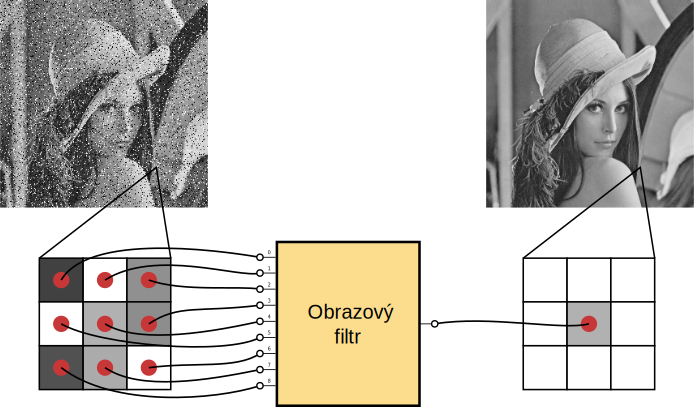
\includegraphics[width=0.66\textwidth]{fig/filter2b.pdf}
    \caption{Princip filtrace obrazu.}
    \label{obrIFokoli}
\end{figure}

Obrazové filtry lze rozdělit na lineární a nelineární. U~lineárních platí princip superpozice a lze je charakterizovat pomocí impulzní odezvy. Výsledný obraz je dán konvolucí vstupního obrazu a impulzní odezvy -- na konvoluci lze nahlížet jako vážený součet zvoleného okolí pixelu. Nevýhodou lineárních filtrů je ztráta detailů. V~jejich případě není výsledný obraz dán konvolucí, ale nějakou nelineární funkcí, například mediánem hodnot okolních pixelů.

Existují různé typy šumů, pro které jsou vhodné různé typy obrazových filtrů. Poměrně častý je impulzní šum, který vzniká kvůli nefunkčním pixelům v~kameře, chybným paměťovým buňkám nebo chybám při přenosu dat. Poškozené body mají buď mají vždy minimální nebo maximální možnou hodnotu (šum typu sůl a pepř) nebo mají náhodnou hodnotu (výstřelový šum). Pro impulzní šum je vhodný nelineární mediánový filtr, ale při intenzivnějším šumu je kvalita nedostatečná a také dochází ke ztrátě detailů.

\begin{figure}[htb]
    \centering
    \subfigure[Vstupní obrázek]{
        \hskip0.75cm
        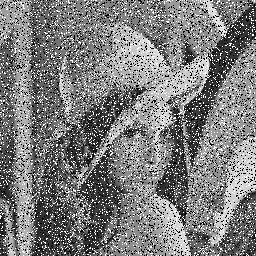
\includegraphics[width=0.21\textwidth]{fig/lena_gray_256_saltpepper_25.png}
        \label{obrSobelIn}
        \hskip0.75cm
    }
    \subfigure[Mediánový filtr s~oknem 3×3]{
        \hskip0.75cm
        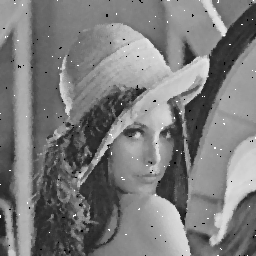
\includegraphics[width=0.21\textwidth]{fig/lena_gray_256_saltpepper_25_median1.png}
        \hskip0.75cm
        \label{obrSobelOut}
    }
    \subfigure[Mediánový filtr s~oknem 5×5]{
        \hskip0.75cm
        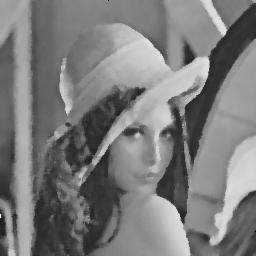
\includegraphics[width=0.21\textwidth]{fig/lena_gray_256_saltpepper_25_median2.png}
        \hskip0.75cm
        \label{obrSobelOut}
    }
    \caption{Výstup mediánového filtru pro obrázek s 25\% šumem typu sůl a pepř.}
    \label{obrDetektor}
\end{figure}

Obrazové filtry se uplatňují i v~jiných úlohách než filtrování šumu. Jedním z~kroků některých algoritmů zpracování obrazu bývá detekce hran. Obrazový filtr má nyní za úkol označit pixely, které jsou ve vstupním obrázku součástí nějaké hrany. Mezi běžně používané detektory hran patří Sobelův nebo Cannyho detektor.

\begin{figure}[htb]
    \centering
    \subfigure[Vstupní obrázek]{
        \hskip0.75cm
        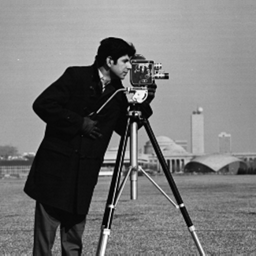
\includegraphics[width=0.21\textwidth]{fig/cameraman_256.png}
        \label{obrSobelIn}
        \hskip0.75cm
    }
    \subfigure[Sobelův detektor]{
        \hskip0.75cm
        
\includegraphics[width=0.21\textwidth]{fig/cameraman_256_sobel.png}
        \hskip0.75cm
        \label{obrSobelOut}
    }
    \subfigure[Cannyho detektor]{
        \hskip0.75cm
        
\includegraphics[width=0.21\textwidth]{fig/cameraman_256_canny.png}
        \hskip0.75cm
        \label{obrSobelOut}
    }
    \caption{Výstup některých detektorů hran.}
    \label{obrDetektor}
\end{figure}



Evoluční algoritmy lze při tvorbě obrazových filtrů využít různými způsoby. Jednou možností je použít již existující obrazový filtr, u~nějž se pomocí genetického algoritmu optimalizuje nastavení jeho parametrů tak, aby se dosáhlo co nejlepších výsledků v~zamýšleném prostředí. Evolučními algoritmy lze také přímo navrhovat nové obrazové filtry. Zvláště výhodné je to u~nelineárních filtrů, pro jejichž analýzu a návrh schází vhodný matematický aparát a jejich tvorba je tak obtížnější než v~případě lineárních filtrů.

Jako vhodné pro tuto úlohu se ukazuje kartézské genetické programování. Na vstup kartézského programu je přivedeno zvolené okolí pixelu, výstupem je filtrovaný pixel. Jako fitness funkce se nejčastěji používá špičková hodnota poměru signál/šum v~decibelech (Peak Signal to Noise Ratio, PSNR) nebo střední odchylka pixelů (Mean Difference Per Pixel, MDPP), která je vhodnější pro hardwarovou implementaci. Tyto funkce jsou definovány:

\begin{equation}
    \label{eqPSNR}
    \mathit{PSNR} = 10 \log_{10} \frac{255^2}{\frac{1}{MN} \sum\limits_{i,j} \left( v\left( i, j \right) - w\left( i, j \right)  \right)^2 }
\end{equation}

\begin{equation}
    \label{eqMDPP}
    \mathit{MDPP} = \frac{1}{MN} \sum\limits_i^M \sum\limits_j^N \left| v\left( i, j \right) - w\left( i, j \right) \right|
\end{equation}

\noindent{}kde $M$ a $N$ označují rozměry obrázku, $v$ filtrovaný a $w$ původní obrázek.

Pro výpočet fitness kandidátního filtru musíme zpracovat celý obrázek, přičemž každý pixel můžeme považovat za jeden případ fitness. Protože i pro poměrně malé obrázky jich je několik tisíc, je výpočet fitness časově velmi náročný \cite{Modra, ZelenaIF}.

\section{Koevoluce v~kartézském genetickém programování}
\label{secCoev}

Jedním ze způsobů, jak řešit problém velkého množství případů fitness je použití koevolučního algoritmu \cite{HandbookCoev}. Oproti dosud zmíněným evolučním algoritmům zde existuje několik různých populací, které na sebe navzájem působí a ovlivňují svůj vývoj. Fitness jedince nezávisí pouze na jeho genetických předpokladech, ale určuje se podle toho, jak \uv{dobrý} je při interakci s~jedinci z~jiných populací.

Populace mohou být stejného druhu. Takové jsou navzájem oddělené bariérou a vyvíjejí se nezávisle na sobě až na občasné migrace jedinců mezi podpopulacemi (například pokud některá z~nich uvízne v~lokálním extrému). V~některých případech je vhodné mít několik populací různého druhu. Některé složitější problémy lze dekomponovat na několik jednodušších, které mohou být reprezentovány různými chromozomy. Jedinci spolu spolupracují na řešení úlohy a jejich kvalita závisí na kvalitě ostatních jedinců. V~tomto případě jde o~\emph{kompoziční koevoluci}.

Další variantou je typ koevoluce, který se používá pro úlohy založené na testu. Populace mezi sebou interagují prostřednictvím fitness funkce, jejíž výsledek závisí i na jedincích okolních populací. V~jedné populaci jsou vyvíjena kandidátní řešení problému, druhá populace obsahuje tzv. \emph{testy}, což jsou podmnožiny množiny případů fitness. Typicky jsou jedinci jedné populace ohodnocování pomocí nejlepšího nebo několika nejlepších jedinců z~jiné populace. Příkladem tohoto typu koevoluce je tzv. \emph{soutěživá koevoluce}, ve které mezi sebou soutěží jedinci ze dvou populací. Cílem populace kandidátních řešení je správně vyřešit všechny případy fitness zahrnuté v~nejlepším testu, naopak cílem populace testů je najít takové případy fitness, ve kterých nejlepší kandidátní řešení selhává. Soutěživou koevoluci poprvé představil Daniel Hillis na úloze návrhu řadicích sítí \cite{Hillis}. Řadicí síť je algoritmus, který řadí posloupnosti dané délky pomocí posloupnosti komparátorů, které mají dva vstupy a výstupy. Komparátor porovnává prvky na vstupy mezi sebou a pokud nejsou v~požadovaném pořadí, na výstupu je zamění. V~soutěživé koevoluci tvoří řadicí sítě populaci kandidátních řešení, druhou populaci testů tvoří neseřazené posloupnosti. Na kandidátní sítě lze nahlížet jako na \uv{hostitele} a na neseřazené posloupnosti jako na \uv{parazity}. Cílem evoluce řadicích sítí je správně seřadit posloupnost v~nejlepším testu, cílem evoluce testů je nalézt takovou neseřazenou posloupnost, která na výstupu sítě není ve správném pořadí.

Koevoluční algoritmy využívají kromě populací i jiný typ množiny jedinců -- tzv. \emph{archivy}, do kterých jsou umisťování nejlepší nalezení jedinci.

Z~implementačního hlediska je možné vyhradit pro každou z~populací samostatné vlákno nebo proces, které mezi sebou komunikují zasíláním zpráv nebo přes sdílenou paměť. Není to ale nutné, koevoluci lze modelovat také tak, že v~každé iteraci algoritmu proběhne několik generací v~první populaci, poté několik generací ve druhé populaci.

Použitím koevoluce CGP a genetického algoritmu lze řešit problém velkého množství případů fitness (zmíněný v~sekci~\ref{secFitnessCalc}).Druhá populace vybírá vhodnou podmnožinu případů fitness, která slouží k~přibližnému určení fitness kandidátních programů \cite{SikuPPSN}.


\subsection{Koevoluční řešení symbolické regrese}

Koevoluční výpočet za účelem snížení výpočetní náročnosti byl poprvé úspěšně ukázán na úloze symbolické regrese \cite{SikuEuroGP}. Zde jsou použity dvě populace: populace kartézských programů (kandidátních řešení symbolické regrese) a populace \emph{prediktorů fitness}. Prediktory jsou podmnožinou množiny případů fitness. Určují, které případy fitness mají být použity k~ohodnocení kandidátních programů. Kromě těchto populací je součástí řešení archiv sdílený oběma populacemi, který obsahuje několik kartézských programů, které slouží pro ohodnocení prediktorů. Celé schéma populací a interakcí mezi nimi znázorňuje obrázek~\ref{obrKoevoluce}.

\begin{figure}[htb]
    \vskip 0.25\baselineskip
    \centering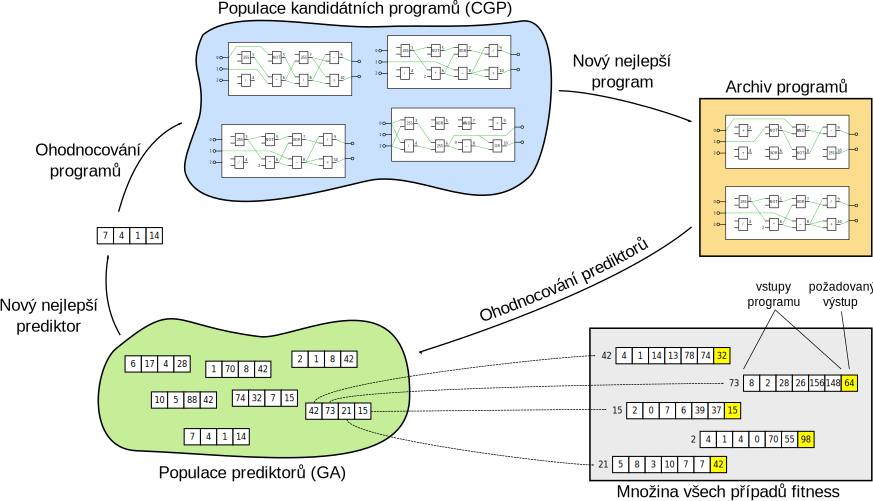
\includegraphics[width=0.9\textwidth]{fig/coev3full.pdf}
    \caption{Schéma koevoluce CGP a prediktorů fitness \cite{SikuEuroGP}.}
    \label{obrKoevoluce}
\end{figure}

Evoluce kandidátních programů probíhá pomocí kartézského genetického programování. Ve skutečnosti existují dvě různé fitness funkce: $f_{\mathit{exact}}$, ve které se používá celá trénovací množina, a $f_{\mathit{predicted}}$, omezená pouze na některé případy fitness.

% Označíme-li kandidátní program jako $s$, velikost trénovací množiny jako $k$ a délku prediktoru fitness (velikost podmnožiny trénovacích dat) jako $m$, můžeme je zapsat následovně:

% \begin{equation}
%     \label{eqFexact}
%     f_{\mathit{exact}} \left( s \right) = \frac{1}{k} \sum\limits_{j=1}^{k} g \left( y \left( j \right) \right)
% \end{equation}

% \begin{equation}
%     \label{eqFpredicted}
%     f_{\mathit{predicted}} \left( s \right) = \frac{1}{m} \sum\limits_{j=1}^{m} g \left( y \left( j \right) \right)
% \end{equation}

Pokud je během evoluce nalezen jedinec s~lepší predikovanou fitness (vypočtenou funkcí $f_{\mathit{predicted}}$) než nejlepší jedinec v~předchozí generaci, je umístěn do archivu sdíleného s~populací prediktorů. Ten je rozdělen na dvě části -- první z~nich obsahuje nejlepší nalezená řešení, do druhé části jsou pravidelně umisťovány náhodně vygenerované programy, čímž je zajištěna větší diverzita jedinců v~archivu. Každý jedinec umístěný do archivu je ohodnocen pomocí celé trénovací množiny (funkcí $f_{\mathit{exact}}$).

Evoluce prediktorů fitness je řízena genetickým algoritmem. Jejich chromozomy jsou vektory ukazatelů do trénovací množiny o~konstantní délce. Potomci jsou tvořeni pomocí jednobodového křížení a mutace, navíc je nejhorší jedinec v~populaci nahrazen náhodně vygenerovaným chromozomem. Fitness prediktoru je určena jako střední absolutní odchylka skutečné a predikované fitness všech programů v~archivu:

\begin{equation}
    \label{eqFpredictorSR}
    f \left( p \right) = \frac{1}{u} \sum\limits_{i=1}^{u} \left| f_{\mathit{exact}} \left( s~\left( i \right) \right) - f_{\mathit{predicted}} \left( s~\left( i \right) \right) \right|
\end{equation}

\noindent{}kde $p$ označuje prediktor a $u$ počet jedinců v~archivu. Prediktor s~nejnižší odchylkou je pak použit pro ohodnocování řešení z~populace kartézských programů.

V~článku \cite{SikuEuroGP} byl tento koevoluční algoritmus porovnán s~běžným CGP na pěti různých funkcích, přičemž trénovací množina pro každou z~nich obsahovala 200 funkčních bodů. Ukázalo se, že koevolucí lze nalézt přijatelné řešení s~použití mnohem menšího počtu evaluací kandidátních programů než u~standardního CGP. Také se ukázalo, že zatímco standardní CGP nenalezlo přijatelné řešení v~23,6\,\% běhů, koevoluční algoritmus byl úspěšný ve všech případech. Co se výpočetní náročnosti týče, byl koevoluční přístup přibližně dvakrát až pětkrát rychlejší, podle hledané funkce.


\subsection{Koevoluční návrh obrazových filtrů}
\label{secCoevIF}

Podobně jako symbolickou regresi lze pomocí koevoluce akcelerovat i evoluční návrh obrazových filtrů. Opět existují dvě populace, kandidátních filtrů v~CGP a podmnožin případů fitness, také je použit sdílený archiv obrazových filtrů. Jednotlivé případy fitness jsou složeny z~devítiokolí poškozeného pixelu a hodnoty téhož pixelu v~původním obrázku (což je očekávaný výstup filtru).

V~článku \cite{SikuPPSN} jsou zmíněny dva různé koevoluční přístupy. V~prvním případě šlo o~koevoluci s~prediktory fitness (CFP, coevolution of fitness predictors), podobně jako u~řešení symbolické regrese popsané výše. Fitness filtrů byla určena pomocí funkce MDPP (viz rovnice~\ref{eqMDPP}), fitness prediktorů pak jako:

\begin{equation}
    \label{eqFpredictorIF}
    f_{\mathit{CFP}} \left( p \right) = \frac{1}{T} \sum\limits_{i=1}^{T} \left| \mathit{MDPP_{exact}} \left( s~\left( i \right) \right) - \mathit{MDPP_{partial}} \left( s~\left( i \right) \right) \right|
\end{equation}

\noindent{}kde $T$ označuje počet položek v~archivu filtrů a $\mathit{MDPP_{partial}}$ je střední odchylka podmnožiny pixelů určených prediktorem, která je dána jako:

\begin{equation}
    \label{eqMDPPPartial}
    \mathit{MDPP_{partial}} = \frac{1}{K} \sum\limits_l^K \left| v\left( l \right) - w\left( l \right) \right|
\end{equation}

\noindent{}kde $K$ označuje počet případů fitness, $v$ filtrovaný a $w$ původní obrázek. Cílem evoluce prediktorů je minimalizace hodnoty fitness.

Ve druhém případě je použita soutěživá koevoluce (CC, competitive coevolution). Podmnožiny případů fitness zde slouží jako jako testy, které reprezentují případy fitness, které kandidátní řešení v~aktuálním stavu koevoluce neumí správně řešit. Cílem filtrů je správně vyřešit všechny případy fitness obsažené v~testu, cílem populace testů je pak najít takové devítiokolí pixelů, které nalezené filtry nejsou schopny vyřešit správně -- tedy nalézt podmnožinu pixelů s~maximalní střední odchylkou filtrované a původní hodnoty. Fitness funkci testů lze odvodit z~rovnice~\ref{eqMDPPPartial} následovně:

\begin{equation}
    \label{eqFtestsIF}
    f_{\mathit{CC}} = \frac{1}{T} \sum\limits_{i=1}^{T} \frac{1}{K} \sum\limits_l^K \left| v\left( l \right) - w\left( l \right) \right|
\end{equation}

Podobně jako u~prediktorů je nejlepší nalezený test použit pro ohodnocení populace filtrů. V~obou variantách jsou nejlepší nalezené filtry umisťovány do archivu, který pak slouží k~ohodnocování prediktorů či testů.

V~porovnání se standardním CGP bylo dosaženo srovnatelné kvality filtrů při použití podmnožiny případů fitness o~velikosti pouze 15\,\% z~celkového počtu pixelů v~obrázku. V~tomto případě byl koevoluční výpočet přibližně třikrát rychlejší než standardní CGP. Oba zmíněné koevoluční přístupy (prediktory fitness i soutěživá koevoluce) vedou na srovnatelně kvalitní filtry \cite{SikuPPSN}.

\subsection{Akcelerace koevolučního návrhu v~hardware}

Koevoluční CGP bylo také úspěšně implementováno v~hardware na rekonfigurovatelném obvodu FPGA. Na úloze návrhu obrazových filtrů, kdy byl měřen čas potřebný na dosažení 10~000 generací CGP, bylo největšího zrychlení dosaženo při použití chromozomů o~délce 25\,\% všech případů fitness, kdy byla hardwarová implementace 58krát rychlejší než optimalizovaná\footnote{Pomocí OpenMP a vektorových (SIMD) instrukcí z~instrukční sady SSE 4.1.} softwarová implementace \cite{Hrbacek}.

\subsection{Návrh obrazových filtrů pomocí kompoziční koevoluce}

Jiným přístupem ke koevolučnímu návrhu je použití kompoziční koevoluce. K~samotnému filtru je možné přidat detektoru šumu, který rozhoduje, zda je právě zpracovávaný pixel poškozený a má být opraven. Cílem je pak nalézt nejlepší kombinaci filtru a detektoru šumu. Experimentálně bylo ověřeno, že koevoluční algoritmus vede na kvalitnější filtry oproti oddělené evoluci filtrů a detektorů šumu bez vzájemné interakce \cite{SikuKomjathy}.

\subsection{Otevřené problémy koevoluce}
\label{secProblems}

Jak bylo ukázáno, použitím koevoluce lze zkrátit dobu potřebnou pro nalezení přijatelného řešení, v~některých případech až pětinásobně. Koevoluční algoritmy dokonce poměrně spolehlivě nachází řešení v~případech, kdy standardní CGP selhává. Na druhou stranu je zapotřebí poměrně velké množství běhů k~nalezení ideálního nastavení. Kromě velikosti populací nebo počtu kandidátních řešení v~archivu jde zejména o~délku chromozomu prediktorů fitness. Ukazuje se, že pro různé úlohy je vhodná jiná hodnota. Při suboptimální konfiguraci pak nemusí být dosaženo takového urychlení výpočtu, jako by bylo možné, anebo kvalita nalezených řešení nemusí být přijatelná. Například v~případě úlohy symbolické regrese bylo potřeba provést více než sto tisíc nezávislých běhů, než bylo nalezeno nejvhodnější nastavení \cite{SikuEuroGP}.

Pokud jsou v~genetickém algoritmu použity dlouhé chromozomy čítající tisíce genů, vyvstává problém škálovatelnosti. U~evolučních algoritmů se pod tímto pojmem rozumí situace, kdy evoluce nenachází přijatelná řešení pro rozsáhlejší úlohy, ačkoliv v~menším měřítku funguje dobře \cite{SikuKomjathy}. Také použití genetických operátorů na příliš dlouhé chromozomy může být neefektivní.

%Tento problém se výrazně projeví například u~permutačně kódovaného chromozomu, kdy se používají speciální genetické operátory modifikující pouze pořadí jednotlivých genů a ne jejich hodnoty .

\subsection{Nepřímo kódované prediktory fitness}
\label{secIndirectPredictors}

Jedním ze způsobů, jak obejít nutnost najít nejvhodnější délku prediktoru pro konkrétní úlohu, je jejich nepřímé kódování, které evoluci umožní tvořit prediktory různé délky a adaptovat je na konkrétní trénovací data. Prediktory nejsou reprezentovány jako vektor ukazatelů do trénovací množiny, ale jako funkce generující posloupnost ukazatelů, které se mají použít při výpočtu fitness.

Pro hledání vhodné funkce je možné použít kartézské genetické programování \cite{SikuHulva}. Funkce je reprezentována jako program s~jedním vstupem a dvěma výstupy. Součástí chromozomu je oproti standardnímu CGP ještě hodnota $x_0$ udávající první vstup programu, pomocí které je získán první prvek posloupnosti. Jeden z~výstupů slouží jako další prvek posloupnosti (a zároveň jako nový vstup programu), druhý pak udává, zda má být posloupnost ukončena. Fitness generátoru závisí kromě odchylky predikované a skutečné fitness také na délce generované posloupnosti -- delší posloupnost vede na větší výpočetní náročnost.

Během experimentů na úloze symbolické regrese se ukázalo, že počet použitých případů fitness odpovídá počtu zjištěnému experimentálně s~přímo kódovanými prediktory. Je tedy možné použít koevoluci s~prediktory fitness na nové úlohy bez časově náročného hledání optimálního nastavení.


\section{Vztah učení a evoluce}
\label{secColearning}

Vztahem mezi učením a evolucí se zabýval už James Mark Baldwin na konci 19. století. Ve svém článku \cite{Baldwin} se zabýval vývojem komplexního instinktivního chování. \emph{Baldwinův efekt} popisuje, jakým způsobem lze postupným vývojem po menších krůčcích dosáhnout komplexních instinktů zakódovaných v~genotypu. Jedinec, jehož instinkt daný genotypem není dokonalý, jej může učením během života zdokonalit a zvýšit tak svou fitness a pravděpodobnost, že i nedokonalý instinkt se přenese na další generaci. Učení má ovšem i své nevýhody, například v~přírodě hrozí, že se během experimentování jedinec zraní nebo zemře, proto jsou upřednostňováni jedinci, kteří mají v~genotypu zakódované dokonalejší instinkty, čímž se postupně vytváří komplexní instinkt \cite{HowToShiftBias}.

\subsection{Plasticita fitness}
\label{secPlasticity}

Schopnost jedince přizpůsobit se prostředí se označuje jako \emph{plasticita fitness} nebo \emph{plasticita fenotypu}. Fenotyp plastického jedince nezáleží jen na genotypu, ale také na okolním prostředí. Jinými slovy, stejný genotyp může tvořit různé fenotypy. V~různých fázích evoluce jsou preferováni jedinci s~různou plasticitou. Po radikální změně prostředí jsou ve výhodě plastičtější jedinci, kteří se změně dokáží lépe přizpůsobit, protože mají větší schopnosti učení. Později, když se prostředí opět ustálí, jsou upřednostňování jedinci, kteří mají nově potřebné vlastnosti přímo zakódované do genotypu. Tento průběh znázorňuje obrázek~\ref{obrBaldwin}.

Různou míru plasticity lze pozorovat nejen mezi jedinci v~populaci, ale také se mění během života jedince. V~průběhu života existují \emph{senzitivní období}, během kterých mají vnější stimuly zvlášť velký význam pro rozvoj jedince -- v~tomto období má vyšší plasticitu. Například pokud bylo kotěti sešito jedno oko, bylo v~dospělosti na něj slepé i po jeho otevření, protože absence vizuálních podnětů v~senzitivním období znemožnila jeho zdravý vývoj. Z~tohoto plyne, že učící aparát je udržován pouze po určitou dobu, nezbytnou pro osvojení příslušné schopnosti.

Přítomnost nebo nepřítomnost schopnosti učení závisí i na dynamice okolního prostředí. Podle četnosti změn v~prostředí lze odlišit několik různých situací. V~případě velmi stabilního prostředí schopnost učení není tolik potřebná a vlastnosti jedince mohou být přímo součástí genotypu. V~opačném případě, kdy ke změnám dochází velmi často je také učení zbytečné, protože neexistují dlouhodobě platná pravidla, které by se jedinec mohl naučit. Mezi těmito extrémy lze pozorovat různou míru plasticity jedinců. Pokud je četnost změn nižší, spíše se projevuje Baldwinův efekt a naučené chování se v~dalších generacích stává součástí genotypu. Se zvyšující se četností změn se objevují senzitivní období na začátku života jedince, od určitého okamžiku pak je schopnost učit se přítomna neustále \cite{EllefsenBalancing}.

\begin{figure}[htb]
    \centering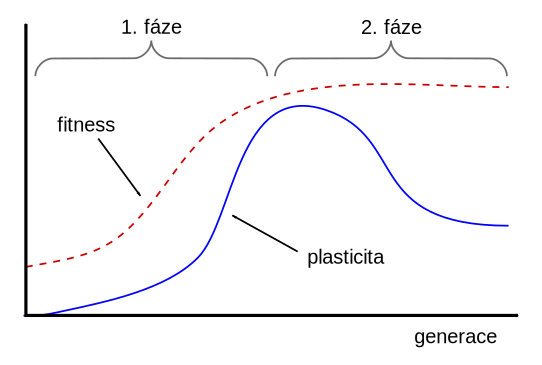
\includegraphics[width=0.5\textwidth]{fig/baldwinPlasticity.pdf}
    \caption{Baldwinův efekt -- nejprve jsou upřednostňování plastičtější jedinci, později převáží cena učení a plasticita klesá \cite{EllefsenBalancing}.}
    \label{obrBaldwin}
\end{figure}

\subsection{Baldwinův efekt v~evolučních algoritmech}

První výpočetní model Baldwinova efektu představili Geoffrey Hinton a Steven Nowlan \cite{HintonNowlan}. Pracovali s~populací jedinců o~20 genech, které mohly nabývat hodnoty \textbf{0}, \textbf{1} nebo \textbf{?}. Genotyp je interpretován jako nastavení 20 spínačů. Alely \textbf{1} a \textbf{0} znamenají, že je příslušný spínač zapnut nebo vypnut, pokud gen obsahuje hodnotu \textbf{?}, může jedinec se spínačem experimentovat. Cílem bylo sepnout všechny spínače. V~případě, že některý gen byl nastaven na \textbf{0}, měl jedinec minimální fitness ($f = 1$), pokud byly všechny geny nastaveny na \textbf{1}, získal jedinec maximální fitness ($f = 20$). Jedinci s~\uv{otazníkovými} alelami měli 1~000 pokusů na nalezení správného řešení a jejich fitness byla úměrná počtu pokusů, které vyčerpali ($f = 1 + 19 \frac{1000 - i}{1000}$, $i$ je počet využitých pokusů). Po 50 generacích se ukázalo, že jedinci mají v~průměru 11 genů nastavených na \textbf{1} a 9 genů na \textbf{?} a průměrnou fitness $f = 11,6$. \uv{Nulové} geny byly poměrně rychle eliminovány. Bez užití učení (a \uv{otazníkových} alel) je očekávaná fitness $f = 1$, protože pravděpodobnost vzniku jedince se všemi geny nastavenými na \textbf{1} je velmi malá a fitness funkce nedokáže odlišit, který jedinec je lepší a který horší (každý má buď maximální nebo minimální fitness), jak znázorňuje obrázek~\ref{obrHintonNowlan}. Přidáním učení se fitness funkce \uv{vyhladí}.

\begin{figure}[htb]
    \centering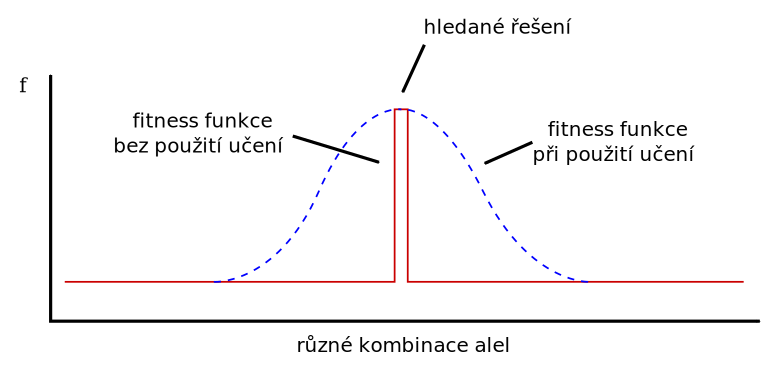
\includegraphics[width=0.68\textwidth]{fig/baldwin1.pdf}
    \caption{Fitness funkce z~experimentu Hintona a Nowlana \cite{HintonNowlan}.}
    \label{obrHintonNowlan}
\end{figure}

Byly představeny také modifikace kartézského genetického programování využívající plastických jedinců.
V~jedné z~nich chromozom obsahoval oproti standardnímu CGP jeden primární výstup navíc, který nebyl přímou součástí kandidátního řešení. U~nově vzniklých potomků je nejprve vytvořen fenotyp, který je posléze modifikován, dokud tento výstup není roven předem stanovené hodnotě. Fitness jedince je pak určena až pomocí modifikovaného fenotypu. V~experimentech na klasifikačních úlohách se ukázalo, že oproti standardnímu CGP lze dosáhnout menší chybovosti \cite{UllahPlasticCGP}.

V~jiné variantě plastického kartézského genetického programování byly z~chromozomu odstraněny geny kódující  propojení primárních výstupů na funkční bloky. Nově vzniklý jedinec pak pro každý primární výstup hledá nejvhodnější funkční blok, tak aby dosáhl co nejvyšší fitness. Na úloze návrhu úplné sčítačky se ukázalo, že algoritmus končí úspěšně bez ohledu na velikost kartézské mřížky, zatímco u~standardního CGP úspěšnost s~větší mřížkou klesala \cite{KhatirPlasticCGP}.

\chapter{Návrh obrazových filtrů pomocí souběžného učení}
\label{chDesign}

Cílem této práce je navrhnout systém pro tvorbu obrazových filtrů založený na principech evolučních algoritmů, koevoluce a souběžného učení. Tento systém bude implementován a experimentálně vyhodnocen v~rámci diplomové práce.

Jedním z~nedostatků koevoluce s~prediktory fitness, popsané v~podkapitole~\ref{secCoevIF}, je nutnost zvolit vhodnou velikost podmnožiny případů fitness, kterou vybírají prediktory. Tato velikost by měla být co nejmenší, aby byl počet nutných vyhodnocení co nejnižší (a výpočet co nejrychlejší), ale zároveň taková, aby odchylka mezi predikovanou a skutečnou fitness kandidátních řešení byla stále přijatelně nízká. Velikost vhodná pro jednu úlohu nemusí být vhodná pro jinou. Například v~případě symbolické regrese mohou u~jednoduchých rovnic stačit pouze jednotky trénovacích vektorů, u~obrazových filtrů to mohou být i tisíce. Někdy je pro stanovení optimální délky nutné provést velké množství experimentů s~různým nastavením; mohou to být i tisíce nezávislých běhů.

Další slabinou koevolučního návrhu je i problém škálovatelnosti -- u~složitějších úloh, jako je návrh obrazových filtrů, může prediktor čítat tisíce genů. Práce s~takto velkými genotypy je pak poměrně neefektivní.

Tyto nedostatky lze obejít použitím jiného kódování prediktorů, kdy nekóduje přímo ukazatele do množiny všech případů fitness, ale pouze návod, podle kterého se mají případy fitness vybírat. V~části~\ref{secIndirectPredictors} je popsáno kódování prediktorů jako programy tvořené dle principů kartézského genetického programování, které generují posloupnost ukazatelů do množiny případů fitness, která může nabývat různé délky.

Tato práce se zabývá novým přímým kódováním prediktorů, jehož cílem je zmírnit současné nedostatky koevoluce pomocí souběžného učení. Pokud umožníme tvorbu různě velkých prediktorů z~jednoho genotypu, mohou jedinci získanou plasticitu využít pro adaptaci na složitost právě řešené úlohy i na aktuální průběh evoluce.

Tato kapitola se nejprve v~části~\ref{secDesignIF} zabývá genotypem a fenotypem obrazových filtrů, následující část~\ref{secDesignEvoSimple} pak samotným průběhem evoluce bez použití koevoluce. Kapitola~\ref{secDesignCoev} popisuje koevoluci CGP a prediktorů fitness. Poslední část~\ref{secDesignColearn} uvádí nové kódování prediktorů fitness s~plastickým fenotypem a možnostmi, jak lze získanou plasticitu využít pro adaptaci prediktorů na průběh evoluce.

\section{Kandidátní obrazové filtry}
\label{secDesignIF}

Obrazové filtry jsou vyvíjeny pomocí kartézského genetického programování, popsaného v~kapitole~\ref{secCGP}. Chromozom tvoří vektor celých čísel kódující acyklický orientovaný graf. Jednotlivé funkční bloky jsou tvořeny trojicí genů -- první z~nich označuje prováděnou funkci, druhý a třetí gen pak určují, kam jsou připojeny jeho vstupy. Seznam funkcí, které mohou výpočetní uzly realizovat je v~tabulce~\ref{tabCGPFunctions}. Programy mají devět primárních vstupů a jeden primární výstup. Na vstupy jsou přiváděny hodnoty pixelů z~devítiokolí právě zpracovávaného pixelu, výstup udává novou hodnotu pixelu, jak je popsáno v~kapitole~\ref{secIF}. V~devítiokolích pixelů na okraji obrázku se na pozicích mimo obrázek používá hodnota nejbližšího okrajového pixelu.

\begin{table}[htb]
    \caption{Seznam funkcí výpočetních uzlů. Převzato z~článku \cite{SikuPPSN}.}
    \renewcommand{\arraystretch}{1.2}
    \begin{minipage}[t]{.5\textwidth}
        \small\centering\begin{tabular}{cll}
            \toprule
            \# & funkce & popis \\
            \midrule
            0 & $255$ & konstanta \\
            1 & $i_1$ & identita \\
            2 & $255 - i_1$ & inverze \\
            3 & $i_1 \vee i_2$ & OR \\
            4 & $\neg i_1 \vee i_2$ & OR s~negovaným vstupem \\
            5 & $i_1 \wedge i_2$ & AND \\
            6 & $\neg (i_1 \wedge i_2)$ & NAND \\
            7 & $i_1 \oplus i_2$ & XOR \\
            \bottomrule
        \end{tabular}

    \end{minipage}
    \begin{minipage}[t]{.5\textwidth}
        \small\centering\begin{tabular}{cll}
            \toprule
            \# & funkce & popis \\
            \midrule
            8 & $i_1 \gg 1$ & posun vpravo o~1 bit \\
            9 & $i_1 \gg 2$ & posun vpravo o~2 bity \\
            10 & $\mathrm{swap}(i_1, i_2)$ & prohození 4 bitů \\
            11 & $i_1 + i_2$ & sčítání \\
            12 & $i_1 +^S i_2$ & saturované sčítání \\
            13 & $(i_1 + i_2) \gg 1$ & průměr \\
            14 & $\max(i_1, i_2)$ & maximum \\
            15 & $\min(i_1, i_2)$ & minimum \\
            \bottomrule
        \end{tabular}

    \end{minipage}
    \label{tabCGPFunctions}
\end{table}

Protože součástí fenotypu nejsou všechny výpočetní uzly, je u~každého funkčního bloku v~chromozomu uložena i informace, zda je aktivní. Pomocí těchto údajů lze urychlit výpočet fitness, protože není nutné počítat výstup neaktivních bloků. V~případě, že jedinec vznikl pouze mutací neaktivních uzlů, není třeba fitness počítat vůbec. Jako fitness funkce je použita špičková hodnota poměru signál/šum (Peak Signal to Noise Ratio):

\begin{equation}
    \label{eqDesignFilterFitness}
    \mathit{f\left(cgp\right)} = 10 \log_{10} \frac{255^2}{\frac{1}{N} \sum\limits_i^N \left( v\left( i \right) - w\left( i \right)  \right)^2 }
\end{equation}

\noindent{}kde $N$ označuje počet použitých případů fitness, $v(i)$ a $w(i)$ pixel filtrovaného (resp. původního) obrázku označený v~množině případů fitness indexem $i$.

\section{Evoluce obrazových filtrů bez koevoluce}
\label{secDesignEvoSimple}

Vstupem algoritmu je zvolený obrázek poškozený šumem (vstup filtru) a týž obrázek v~původní podobě (referenční výstup). Každé devítiokolí pixelů poškozeného obrázku a odpovídající nepoškozený pixel z~originálního obrázku tvoří jeden případ fitness.

Na začátku je náhodně vytvořena počáteční populace a vypočtena fitness všech jedinců. Jedinec s~nejlepší fitness se stává rodičem následující generace. Ostatní jedinci jsou nahrazeni jeho kopiemi a několik jejich genů je pozměněno mutací -- používá se tedy evoluční strategie $(1 + \lambda)$. Mutace dodržuje pravidla zmíněná v~části~\ref{secCGPEvo} s~tím rozdílem, že není povoleno na primární výstup připojit primární vstup. Takto vytvořená populace je opět ohodnocena fitness funkcí a algoritmus pokračuje výběrem rodiče a tvorbou další generace.

Evoluce je ukončena po dosažení předem specifikovaného počtu generací. Volitelně je možné i určit cílovou hodnotu PSNR, po jejímž dosažení bude výpočet ukončen.



\section{Koevoluce obrazových filtrů a prediktorů fitness}
\label{secDesignCoev}

Koevoluce obrazových filtrů a prediktorů pracuje dle principů popsaných v~části~\ref{secCoevIF}. Součástí algoritmu je kromě populace obrazových filtrů také populace prediktorů fitness, která se vyvíjí pomocí genetického algoritmu (viz část~\ref{secGA}). Obě populace interagují prostřednictvím dvou archivů, které obsahují jednak kandidátní filtry a jednak prediktor, který se používá pro ohodnocení filtrů.

\subsection{Fitness kandidátních filtrů}

U~populace obrazových filtrů jsou použity dvě různé fitness funkce. \emph{Skutečná fitness} $f_{\mathit{exact}}$ je určena pomocí celé množiny případů fitness a slouží pro výpočet fitness prediktorů a také pro posuzování průběhu evoluce při modifikaci proměnné \emph{UsedGenes}. Oproti tomu \emph{predikovaná fitness} $f_{\mathit{predicted}}$ používá při výpočtu pouze případy fitness určené prediktorem. Používá se pro ohodnocení jak obrazových filtrů, tak prediktorů. V~obou případech je jako fitness použita hodnota PSNR dle rovnice~\ref{eqDesignFilterFitness}.

\subsection{Prediktory fitness pevné délky}

Chromozom prediktorů je reprezentován jako celočíselný vektor, kdy každý gen je ukazatelem do množiny případů fitness o~konstantní délce, přičemž žádné dva geny nemají stejnou hodnotu. Cílem evoluce je nalézt takové prediktory, u~kterých je odchylka mezi skutečnou fitness $f_{\mathit{exact}}$ a predikovanou fitness $f_{\mathit{predicted}}$ u~všech kandidátních programů v~archivu co nejmenší. Fitness funkci lze zapsat následovně:

\begin{equation}
    \label{eqDesignPredFitness}
    f \left( p \right) = \frac{1}{u} \sum\limits_{i=1}^{u} \left| f_{\mathit{exact}} \left( s\left( i \right) \right) - f_{\mathit{predicted}} \left( s\left( i \right) \right) \right|
\end{equation}

\noindent{}kde $f \left( p \right)$ je fitness prediktoru, $u$ počet filtrů použitých k~ohodnocení prediktoru, $f_{\mathit{exact}}$ označuje skutečnou fitness filtru $s\left( i \right)$ a $f_{\mathit{predicted}}$ predikovanou fitness filtru $s\left( i \right)$.

\subsection{Archivy}

Archiv kandidátních filtrů je reprezentován polem o~pevné délce. Pokud je zaplněn, jsou nejstarší položky přepisovány novými (kruhový buffer). Každý záznam obsahuje chromozom kandidátního filtru a jeho skutečnou fitness. Filtry obsažené v~archivu slouží k~výpočtu fitness prediktorů dle rovnice~\ref{eqDesignPredFitness}.

Archiv prediktorů je tvořen jedinou položkou -- nejlepším nalezeným prediktorem. Ten slouží k~výpočtu predikované fitness při evoluci obrazových filtrů.

\subsection{Průběh evoluce}

Na začátku běhu programu jsou náhodně vytvořeny počáteční populace filtrů a prediktorů fitness. Poté je vypočtena skutečná fitness filtrů a nejlepší jedinec je umístěn do archivu. Pomocí něj jsou ohodnoceny prediktory fitness a je určen nejlepší ten, který bude zpočátku sloužit pro výpočet predikované fitness. Po této inicializaci archivů pokračuje běh programu ve dvou oddělených vláknech, kde každé obsluhuje jednu populaci. Běh programu znázorňuje diagram na obrázku~\ref{obrProgramCoev}.

Evoluce kandidátních filtrů probíhá stejně jako v~případě bez koevoluce (viz část~\ref{secDesignEvoSimple}). Rozdíl je v~tom, že pokud je predikovaná fitness nejlepšího potomka vyšší než fitness jeho rodiče (a stává se tak novým rodičem), je umístěn do sdíleného archivu.

V~populaci prediktorů fitness je nová populace tvořena třemi druhy potomků. Jednu čtvrtinu celkového počtu jedinců tvoří nejlepší jedinci (elitismus). Druhá čtvrtina potomků je vygenerována zcela náhodně, aby se zachovala diverzita populace. Zbývající dvě čtvrtiny potomků jsou tvořeni pomocí jednobodového křížení a mutace, která nahrazuje malé množství genů náhodnými hodnotami. Jejich rodiče jsou voleni pomocí turnaje, ve kterém se každého kola účastní dva náhodně zvolení jedinci. V~případě, že má některý potomek vyšší fitness, než má prediktor v~archivu, nahradí jej.

Evoluce je stejně jako v~případě bez koevoluce ukončena po dosažení stanoveného počtu generací nebo požadované hodnoty PSNR.

\begin{figure}[hb]
    \vskip\baselineskip
    \centering
    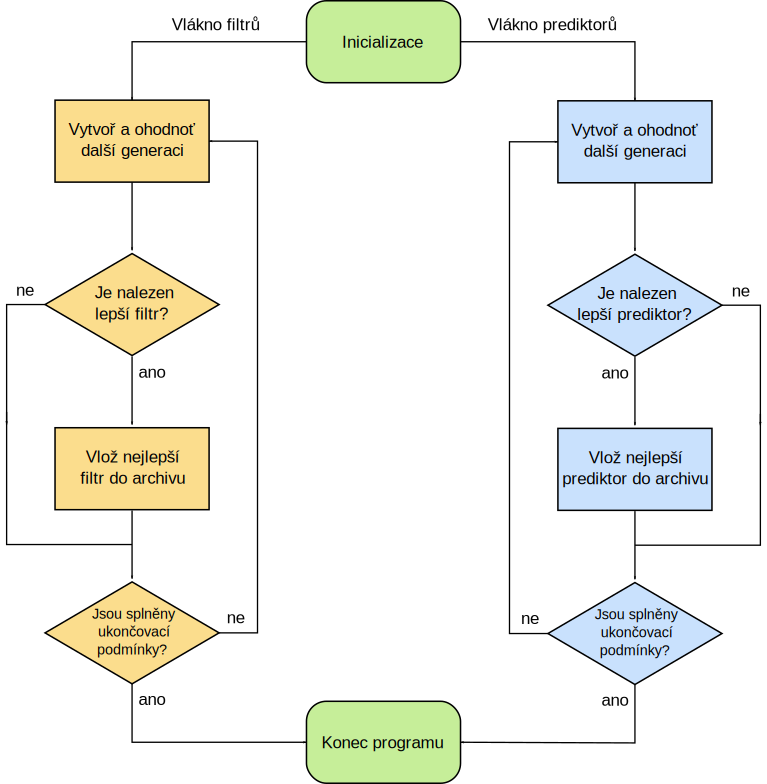
\includegraphics[width=0.75\textwidth]{fig/program}
    \caption{Vývojový diagram koevoluce obrazových filtrů a prediktorů fitness.}
    \label{obrProgramCoev}
\end{figure}



\section{Souběžné učení v~koevoluci filtrů a prediktorů fitness}
\label{secDesignColearn}

V~případě souběžného učení v~koevolučním CGP se používá mírně odlišné kódování prediktorů, které se vyznačuje plastickým fenotypem, což znamená, že lze z~jednoho genotypu odvodit různé fenotypy. V~této části je popsáno, jak toto kódování vypadá a jakým způsobem lze získanou plasticitu využít pro adaptaci prediktorů na složitost řešeného problému v~průběhu evoluce.

\subsection{Plastické prediktory fitness}
\label{secDesignPred}

Chromozom je stejně jako v~případě prediktorů pevné délky reprezentován jako vektor číselných ukazatelů do množiny případů fitness. Rozdíl je v~počtu genů, který zde odpovídá celkovému počtu případů fitness. Ačkoliv ani zde není žádoucí, aby prediktor obsahoval některé ukazatele vícekrát, jsou v~genotypu povoleny duplicitní hodnoty. Zamezit by jim šlo použitím například permutačního kódování, ale to je pro chromozomy o~tisících genech, jenž se dají u~návrhu obrazových filtrů očekávat, už poměrně neefektivní.

Plasticita je dosažena tím, že fenotyp netvoří všechny ukazatele obsažené v~genotypu, ale pouze jejich část. Fenotyp je z~genotypu tvořen postupným čtením genů od zvolené pozice (\emph{offsetu}). Pokud hodnota právě čteného genu není obsažena ve fenotypu, je do něj vložena, v~opačném případě se gen ignoruje. Poté je přečten další gen a proces se opakuje. Během tvorby fenotypu nejsou čteny úplně všechny geny -- jejich počet je určen hodnotou \emph{UsedGenes}, která je součástí prostředí. Pokud je při čtení dosaženo konce genotypu, ale nebyl ještě přečten potřebný počet genů, pokračuje se od jeho začátku. Příklad tvorby fenotypu při použití šesti genů z~deseti ukazuje obrázek~\ref{obrFenotyp}.

\begin{figure}[htb]
    \centering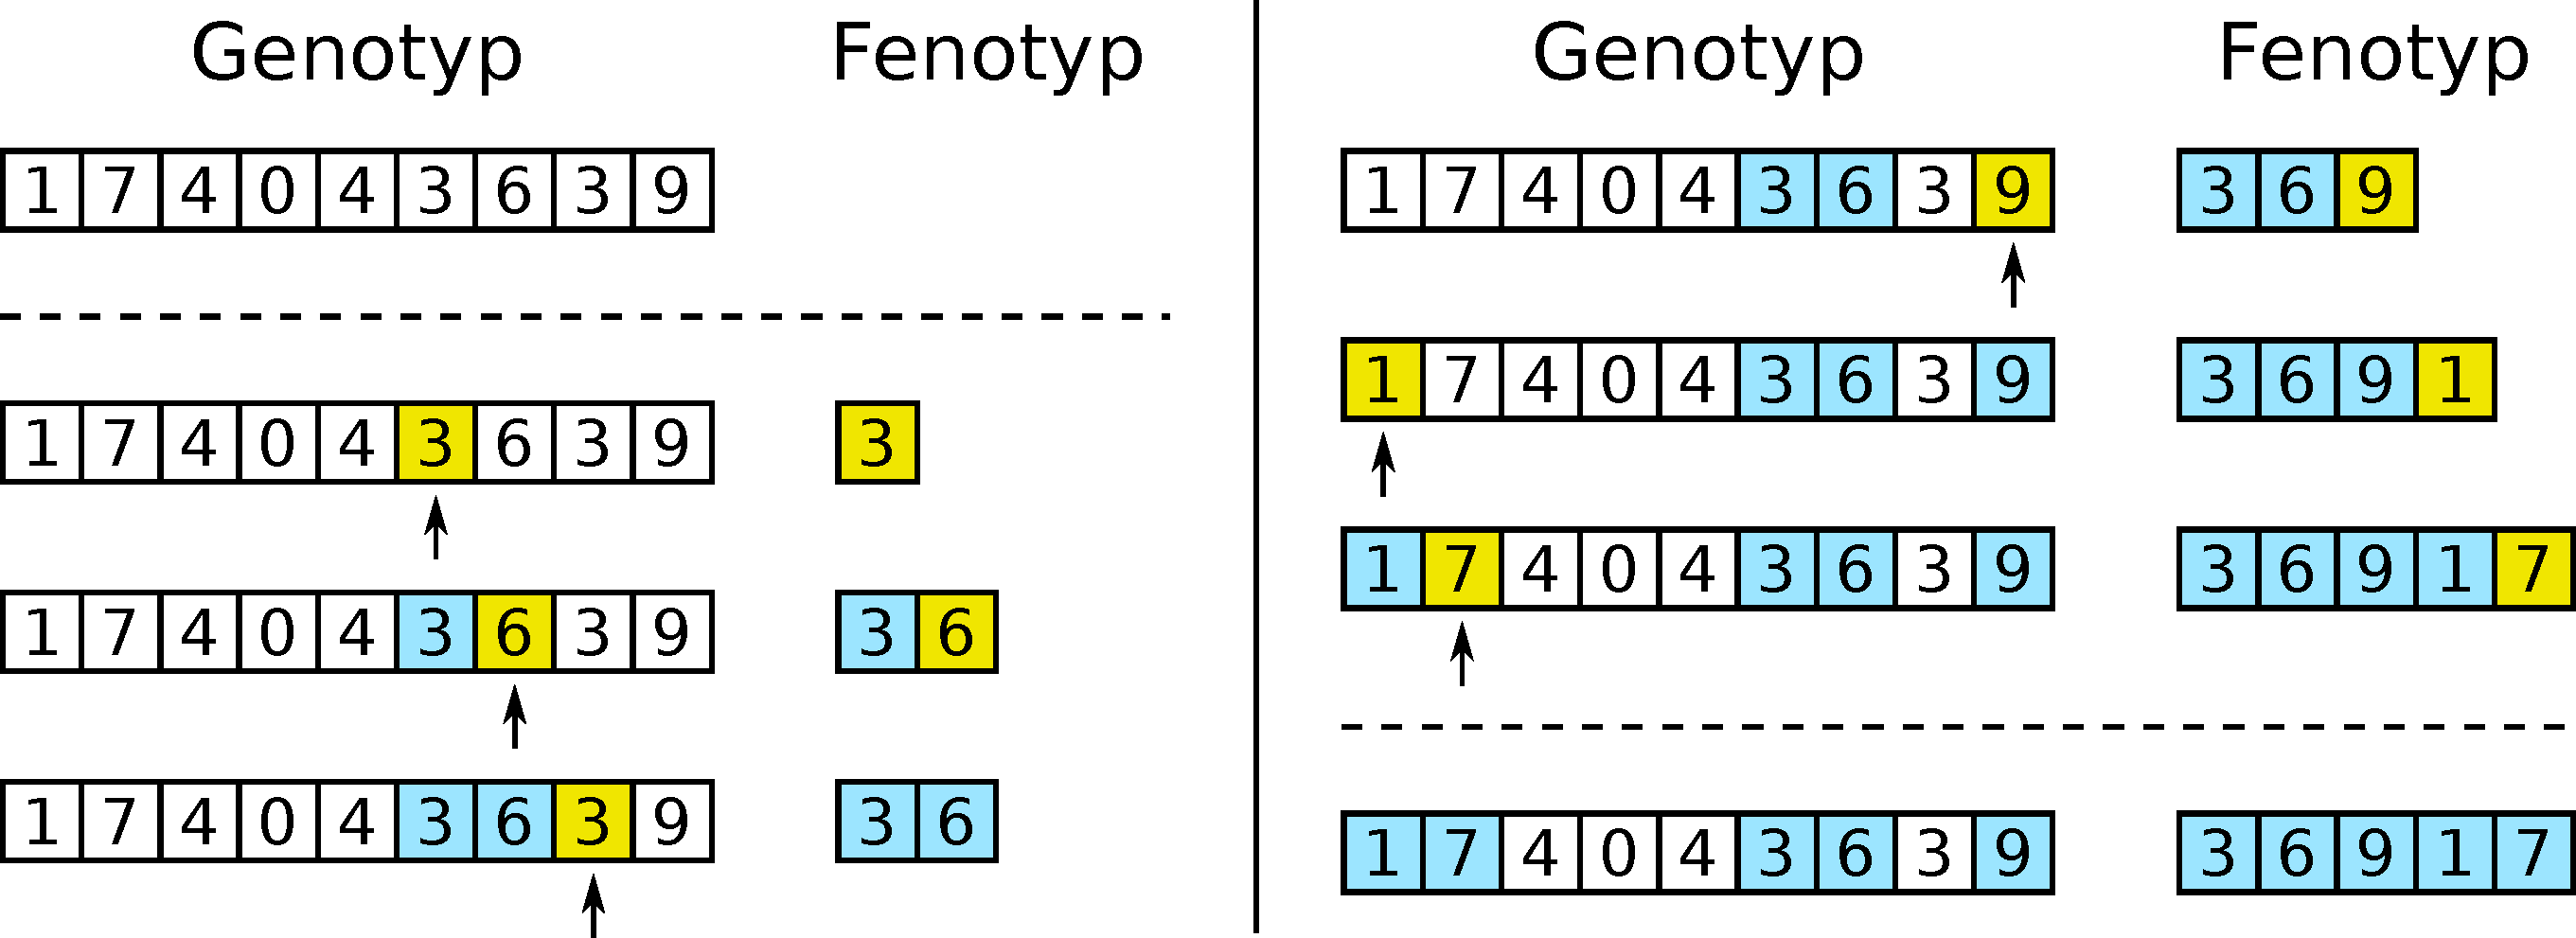
\includegraphics[width=0.9\textwidth]{fig/phenotype2.pdf}
    \caption{Postup konstrukce fenotypu prediktoru. Šipka označuje právě přečtený gen.}
    \label{obrFenotyp}
\end{figure}

S~plasticitou jedinců lze pracovat různými způsoby. Především lze velikost prediktorů adaptovat na průběh evoluce kandidátních filtrů. Další možností je simulovat u~prediktoru učení a adaptaci na prostředí tak, že nově vytvořený prediktor se snaží najít nejvýhodnější offset několika náhodnými pokusy. Také lze v~situaci, kdy evoluce filtrů stagnuje, skokově změnit offset všech prediktorů v~populaci, což může pomoci v~posunu z~lokálního optima. Všechny zmíněné možnosti lze kombinovat.

\subsection{Adaptace velikosti prediktoru na průběh evoluce}
\label{secDesignAdaptation}

Adaptace velikosti prediktoru probíhá na základě sledování rychlosti vývoje skutečné fitness kan\-di\-dát\-ních ře\-šení. Podobně, jako lze pozorovat senzitivní období v~životě jedince (viz kapitola~\ref{secPlasticity}), lze očekávat, že i populace prochází obdobími, kdy je celková schopnost adaptace vyšší (a fitness populace stoupá) a obdobími, kdy se adaptovat příliš nedokáže (a fitness se nemění). Důležitý je i~směr změny fitness, protože je pro ohodnocení je\-dinců v~CGP používána predikovaná fitness a skutečná fitness nejlepšího jedince může i klesat. Rychlost evoluce je možné například určit jako podíl změny fitness nej\-lep\-šího jedince v~populaci a počtu generací, které uběhly od minulé změny:

\begin{equation}
    \label{eqVelocity}
    v~= \frac{\Delta{}f_{\mathit{exact}}}{\Delta{}G}
\end{equation}

Lze pracovat ale i s~delším úsekem historie, například jako celkovou rychlost $v$ použít medián či (vážený) průměr rychlostí za několik posledních změn. Také lze ručně připravit trénovací data sestávající z~několika na sebe navazujících změn a odvodit z~nich vzorec pro výpočet celkové rychlost evoluce, například pomocí symbolické regrese.

U~příliš krátkých prediktorů (v~extrémním případě to může být i jen jeden případ fitness) hrozí, že se velmi dobře adaptují na kandidátní řešení uložená v~archivu a predikce u~jiných filtrů bude velmi nepřesná. Proto se sleduje i nepřesnost predikce a pokud překročí stanovenou mez $I_\mathit{threshold}$, prediktory se prodlouží. Nepřesnost prediktoru lze určit jako poměr mezi predikovanou a skutečnou hodnotou fitness nejlepšího filtru v~populaci:

\begin{equation}
    \label{eqInaccuracy}
    \mathit{I} = \frac{f_{\mathit{predicted}}}{f_{\mathit{exact}}}
\end{equation}

Velikost prediktoru se upravuje vždy při změně rodiče v~populaci filtrů, což v~CGP znamená, že některý z~potomků má vyšší nebo stejnou predikovanou fitness jako jeho rodič. Také lze volitelně nastavit, že změna velikosti musí nastat minimálně jednou za určitý počet generací.

Vždy, když má dojít k~úpravě velikosti prediktoru, je zvolen koeficient, pomocí kterého se upraví současná hodnota proměnné \emph{UsedGenes}, čímž se změní velikost fenotypů prediktorů. Na výběr jsou dva způsoby. Při \emph{relativní} změně se nová hodnota \emph{UsedGenes} získá prostým vynásobením současné hodnoty koeficientem. Ve druhém případě je koeficientem vynásoben celkový počet případů fitness a výsledná hodnota je přičtena k~současné hodnotě \emph{UsedGenes}. Hodnoty koeficientů jsou určeny experimentálně, nicméně základní předpoklady jsou:

\begin{description}
    \item[Koeficient $c_I$:] Pokud je nepřesnost predikce příliš vysoká, prediktory se prodlouží.
    \item[Koeficient $c_{0}$:] Pokud se fitness nemění ($v \approx 0$), evoluce pravděpodobně uvázla v~lokálním optimu, prediktory se zkrátí, čímž mohou pomoci se z~tohoto optima posunout dále.
    \item[Koeficient $c_{-1}$:] Pokud fitness klesá ($v < 0$), evoluce pravděpodobně opouští lokální optimum a mírné zkrácení prediktoru může pomoci postup urychlit.
    \item[Koeficienty $c_{+1}$ a $c_{+2}$:] Pokud fitness roste ($v > 0$), je vhodně prediktory prodloužit, čímž se zpřesní predikce. Rozlišuje se mezi \emph{pomalým} a \emph{rychlým} růstem.
\end{description}

Hraniční rychlost, při které je rychlost evoluce ještě považována za nulovou určuje parametr $v_\mathit{zero}$. V~případě kladné rychlosti se mezi \emph{pomalým} a \emph{rychlým} růstem rozhoduje podle hodnoty parametru rychlý nebo pomalý růst je určen $v_\mathit{slow}$.

Všechna pravidla použitá v~algoritmu shrnuje tabulka~\ref{tabBaldwinRules}. Pokud je splněna podmínka některého z~pravidel, další pravidla v~pořadí se již nevyhodnocují.

\begin{table}[htb]
    \caption{Zvolená pravidla pro změnu velikosti prediktoru.}
    \small\centering
    \renewcommand{\arraystretch}{1.2}
    \subtable[Relativně k~současné velikosti prediktoru]{
        \begin{tabular}{llll}
            \toprule
            \# & podmínka                               & nová hodnota \emph{UsedGenes}     & popis \\
            \midrule
            1. &  $I > I_\mathit{threshold}$            & $\mathit{UsedGenes} \cdot c_I$    & nepřesná predikce     \\
            2. &  $\left|v\right| \leq v_\mathit{zero}$ & $\mathit{UsedGenes} \cdot c_0$    & fitness se nemění     \\
            3. &  $v < 0$                               & $\mathit{UsedGenes} \cdot c_{-1}$ & fitness klesá         \\
            4. &  $0 < v~\leq v_\mathit{slow}$              & $\mathit{UsedGenes} \cdot c_{+1}$ & fitness pomalu stoupá \\
            5. &  $v > v_\mathit{slow}$                 & $\mathit{UsedGenes} \cdot c_{+2}$ & fitness rychle stoupá \\
            \bottomrule
        \end{tabular}
    }
    \vskip0.5\baselineskip
    \subtable[Podle celkového počtu případů fitness $N$]{
        \begin{tabular}{llll}
            \toprule
            \# & podmínka                               & nová hodnota \emph{UsedGenes}                      & popis \\
            \midrule
            1. &  $I > I_\mathit{threshold}$            & $\mathit{UsedGenes} \cdot c_I$                     & nepřesná predikce     \\
            2. &  $\left|v\right| \leq v_\mathit{zero}$ & $\mathit{UsedGenes} + \left(N \cdot c_0\right)$    & fitness se nemění     \\
            3. &  $v < 0$                               & $\mathit{UsedGenes} + \left(N \cdot c_{-1}\right)$ & fitness klesá         \\
            4. &  $0 < v~\leq v_\mathit{slow}$              & $\mathit{UsedGenes} + \left(N \cdot c_{+1}\right)$ & fitness pomalu stoupá \\
            5. &  $v > v_\mathit{slow}$                 & $\mathit{UsedGenes} + \left(N \cdot c_{+2}\right)$ & fitness rychle stoupá \\
            \bottomrule
        \end{tabular}
    }
    %Hodnoty $c_I$, $c_0$, $c_{-1}$, $c_{+1}$, $c_{+2}$, $v_\mathit{zero}$ a $v_\mathit{slow}$ jsou parametry algoritmu.
    \label{tabBaldwinRules}
\end{table}



%\begin{itemize}
%    \item Pokud fitness stoupá, je vhodné prodloužit prediktory a tím zpřesňovat predikci.
%    \item Pokud se fitness nemění, evoluce pravděpodobně uvázla v~lokálním optimu a kratší prediktory mohou pomoci se z~tohoto optima posunout dále.
%    \item Pokud fitness klesá, evoluce pravděpodobně opouští lokální optimum a mírné zkrácení prediktoru může pomoci postup urychlit.
%\end{itemize}

% Velikost prediktoru lze upravovat buď relativně k~současné délce vynásobením současné délky vhodným koeficientem, nebo přičtením či odečtením hodnoty určené relativně k~celkovému počtu případů fitness. V~různých situacích je použit jiný koeficient: %Pomocí jednoduchých pravidel je   pracují s následujícími parametry, které určují, jak se má změnit velikost prediktoru:

% \begin{itemize}
%     \item $c_I$ při nepřesné predikci,
%     \item $c_0$ při neměnné fitness filtrů,
%     \item $c_{-1}$ při klesající fitness filtrů,
%     \item $c_{+1}$ při rostoucí fitness filtrů, pokud je rychlost nižší než hodnota parametru $v_\mathit{slow}$,
%     \item $c_{+2}$ při rychlosti vyšší než $v_\mathit{slow}$.
% \end{itemize}


%Celkem jde o pět parametrů: $c_I$ (nepřesná predikce), $c_0$ (neměnná fitness), $c_{-1}$ (klesající), $c_{+1}$ (pomalu rostoucí) a $c_{+2}$ (rychle rostoucí).

\subsection{Paměť průběhu evoluce}
\label{secDesignHistory}

Aby bylo možné vypočítat rychlost evoluce kandidátních filtrů, je potřeba udržovat historii fitness rodičů delší, než jen mezi aktuální a novou generací. Protože není potřeba udržovat celou historii, ale zajímá nás jen poslední vývoj, jsou nejstarší položky přepisovány novějšími -- z~implementačního pohledu jde o~kruhový buffer. Ukládá se zejména:

\begin{itemize}
    \item $\Delta{}f_{\mathit{exact}}$ -- rozdíl skutečné fitness filtrů oproti poslednímu záznamu,
    \item $\Delta{}G$ -- počet uběhlých generací,
    \item $\frac{\Delta{}f_{\mathit{exact}}}{\Delta{}G}$ -- \uv{rychlost} evoluce (průměrná změna fitness na jednu generaci).
\end{itemize}

Nová položka je do paměti vložena vždy, když je predikovaná fitness nejlepšího potomka vyšší, než byla u~jeho rodiče. Volitelně mohou být záznamy tvořeny v~pravidelných intervalech, například každých tisíc generací. V~tomto případě je možné, že fitness bude delší dobu stejná a kruhový buffer již nebude obsahovat informaci o~směru poslední změny. Proto paměť obsahuje zvláštní pozici pro poslední záznam s~nenulovým rozdílem fitness, která není součástí kruhového bufferu.


% \begin{equation}

%     \mathit{UsedGenes} \leftarrow \left\{
%         \begin{array}{ll}
%             \mathit{UsedGenes} \cdot k_I    & \mbox{pokud } I > I_\mathit{threshold} \\
%             \mathit{UsedGenes} \cdot k_0    & \mbox{pokud } \left|v\right| \leq v_\mathit{zero} \\
%             \mathit{UsedGenes} \cdot k_{-1} & \mbox{pokud } v < -v_\mathit{zero} \\
%             \mathit{UsedGenes} \cdot k_{+1} & \mbox{pokud } v_\mathit{zero} < v \leq v_\mathit{fast}   \\
%             \mathit{UsedGenes} \cdot k_{+2} & \mbox{pokud } v > v_\mathit{fast}   \\
%         \end{array}
%     \right.
% \end{equation}



\subsection{Průběh evoluce}

V~případě souběžného učení probíhá evoluce stejně, jako u~koevolučního CGP. Hlavní rozdíl je v~prováděných akcích po nalezení filtru s~lepší predikovanou fitness, než měl jeho rodič. V~takovém případě je navíc do paměti průběhu evoluce vložen nový záznam a upraví se hodnota \emph{UsedGenes}, čímž se změní velikost fenotypu prediktorů. K~úpravě hodnoty \emph{UsedGenes} může dojít také po stanoveném počtu generací CGP, během kterých nebyl nalezen lepší obrazový filtr.

\section{Paralelizace programu}
\label{secDesignParallel}

V~navrženém programu lze některé činnosti provádět paralelně. Jde například o~souběžnou evoluci populace filtrů a populace prediktorů, výpočet fitness jedinců a tvorbu potomků (filtrů i prediktorů), jednotlivá kola turnajové selekce rodičů v~populaci prediktorů nebo výpočet výstupů kandidátního filtru pro různé případy fitness. Také výpočet skutečné fitness programů uložených do archivu může probíhat v~samostatném vlákně.

V~případě koevoluce (a souběžného učení) se program po inicializaci rozdělí do dvou vláken, v~prvním z~nich probíhá evoluce obrazových filtrů, ve druhém evoluce prediktorů fitness. Jejich běh není synchronizován, evoluce na sebe \uv{nečekají}. Vlákna mezi sebou komunikují prostřednictvím sdílené paměti, ve které jsou uloženy především archivy s~kandidátními programy a s~nejlepším nalezeným prediktorem. Pokud se používá souběžné učení, obsahuje sdílená paměť navíc historii změn fitness nejlepšího programu (viz část~\ref{secDesignHistory}).

Přístup ke sdíleným proměnným musí být ošetřen vhodným synchronizačním mechanismem, aby nedocházelo k~nežádoucím chybám (\emph{race-conditions}). V~případě, že je do archivů kopírován nový kandidátní filtr nebo prediktor, nemůže druhé vlákno ohodnocovat potomky. Při použití souběžného učení navíc nelze během změny velikosti prediktorů a následném přepočtu jejich fitness s~novým fenotypem ohodnocovat obrazové filtry ani vkládat nové kandidátní filtry do archivu.

Koevoluci lze implementovat také pseudo-paralelně, kdy se obě populace periodicky střídají~-- po uplynutí stanoveného počtu generací populace filtrů se provede několik generací populace prediktorů. Sice odpadá nutnost ošetřování přístupu ke sdíleným proměnným, program by ale byl pomalejší.

Rozhodl jsem se výpočet skutečné fitness nevyčleňovat do samostatného vlákna, probíhá tedy v~rámci vlákna zpracovávající evoluci filtrů ihned po uložení programu do archivu.

Kromě těchto dvou vláken se běh programu dělí na další vlákna během ohodnocování jedinců a tvorbě potomků. Schéma paralelizace při použití koevoluce je na obrázku~\ref{obrParalelizace}. U~standardního CGP není potřeba na začátku běhu programu vytvářet vlákna pro evoluci populací. Výpočet fitness a tvorba potomků probíhá paralelně stejně jako u~koevoluce.

Ukončovací podmínky se kontrolují ve vlákně evoluce filtrů. Druhému vláknu je konec běhu signalizován prostřednictvím sdílené proměnné \texttt{finished}.

\begin{figure}[htb]
    \centering
    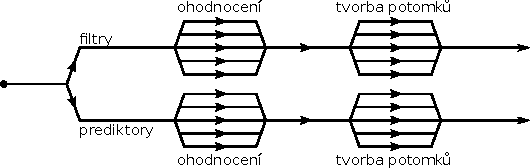
\includegraphics[width=0.75\textwidth]{fig/openmp}
    \caption{Rozdělení běhu programu na vlákna při použití koevoluce. U~standardního CGP se program na začátku nedělí do dvou paralelních sekcí.}
    \label{obrParalelizace}
\end{figure}


\chapter{Implementace navrženého algoritmu}
\label{chImplementation}

Kvůli velkému množství plánovaných experimentů byl kladen důraz především na co nejrychlejší běh programu. Implementován byl proto v~jazyce C, ve kterém lze snadno pracovat i s~assemblerem a rozšiřujícími instrukčními sadami procesoru. U~některých částí algoritmu se nabízí využít nějakou formu paralelizace, jde například o~souběžný běh obou populací, ohodnocování a tvorbu jedinců nebo výpočet výstupu kandidátního filtru.

V~implementaci se využívá některých vlastností normy C11 (například podpora zarovnání dat v~paměti), ale většina využitých vlastností je definována i ve standardu POSIX, i když někdy trochu jiným způsobem. Dle použitého překladače se pak pomocí maker preprocesoru vybere dostupná implementace.

Tato kapitola se nejprve v~části~\ref{secImplParalelization} zabývá paralelizací evoluce na úrovni populací a jedinců. Část~\ref{secImplVectorization} popisuje optimalizací výpočtu výstupů filtrů pomocí vektorových (SIMD) instrukcí a úpravy, které jsou potřeba pro efektivní vektorizaci. Následující část~\ref{secImplImages} se zabývá práci s~obrázky a poslední část~\ref{secImplExperimental} programovou podporou pro experimentální vyhodnocení.

\section{Paralelizace evoluce}
\label{secImplParalelization}

Navržený program lze v~některých částech výpočetu paralelizovat, jak je uvedeno v~části~\ref{secDesignParallel}. Na výběr je několik možností, jak paralelní zpracování implementovat. Lze využít prostředků operačního systému a běh programu rozdělit na vlákna nebo podprocesy, ale je to poměrně pracné. Existují knihovny, pomocí kterých lze pracovat na vyšší úrovni abstrakce. Zejména jde o~standardy \emph{Message Passing Interface} (MPI)\footnote{Implementovaný například v~knihovně OpenMPI (\url{http://www.open-mpi.org/}).} a \emph{OpenMP}\footnote{\url{http://openmp.org/}}. Zatímco MPI je založeno na zasílání zpráv mezi výpočetními uzly (např. v~počítačovém clusteru), OpenMP je zaměřeno na paralelizaci se sdílenou pamětí. Lze je i mezi sebou kombinovat, například MPI může sloužit pro rozdělení výpočtu mezi jednotlivé uzly a OpenMP pro paralelizaci v~rámci jednoho uzlu \cite{Quinn}.

%Rozhodl jsem se použít pouze OpenMP.

\subsection{Implementace pomocí OpenMP}

Standard OpenMP definuje speciální direktivy překladače pro označení paralelních částí programu v~jazyce FORTRAN, C nebo C++. Také poskytuje několik knihovních funkcí a proměnných prostředí, pomocí kterých lze zjišťovat nebo upravovat nastavení běhu, například maximální počet používaných vláken. Při použití OpenMP se programátor vůbec nemusí zabývat samotnou implementací paralelizace na nejnižší úrovni. Také se nemusí zabývat případnými rozdíly v~implementaci vláken na různých platformách. Veškerý nízkoúrovňový kód vygeneruje překladač. Také lze ze stejného zdrojového kódu vytvořit sekvenční verzi programu prostým ignorováním direktiv OpenMP \cite{Quinn}.

Při spuštění programu lze parametry příkazové řádky určit, zda se má použít koevoluce nebo pouze standardní CGP. V~prvním případě je po inicializaci program rozdělen do dvou paralelních sekcí (direktivou \texttt{\#pragma omp parallel sections}). V~každé z~nich se pak vyvíjí jedna populace. Přístupy ke sdílené paměti, která obsahuje archivy s~kandidátními programy a s~nejlepším nalezeným prediktorem, jsou uzavřeny do kritických sekcí (\texttt{\#pragma omp critical}). Jinak není běh obou populací nijak synchronizován. Rozdělení jedinců mezi vlákna při výpočtu fitness zajišťuje direktiva \texttt{\#pragma omp parallel for}. Po určení rodičů je stejným způsobem paralelizována i tvorba potomků a nové populace.

V~případě souběžného učení se nová délka prediktoru počítá ve vlákně populace CGP, ačkoliv samotná změna velikosti se provádí ve vlákně prediktorů (ihned po vytvoření nové generace prediktorů). Je to z~toho důvodu, že během jedné generace prediktorů může proběhnout i několik generací CGP, a v~případě, že by se nová velikost počítala ve vlákně prediktorů, nebyly by zahrnuty některé změny nejlepší fitness filtrů.

V~případě, že na cílové platformě není dostupný překladač s~podporou OpenMP, nelze spustit koevoluci. Toto by bylo možné obejít pseudo-paralelní implementací, touto variantou jsem se ale nezabýval. Program tak lze používat jen se standardním CGP, ale ohodnocování jedinců a tvorba potomků bude probíhat sekvenčně.


\section{Vektorizace výpočtu CGP}
\label{secImplVectorization}

Největší důraz byl kladen na optimalizaci rychlosti výpočtu výstupních hodnot kartézských programů, což je časově nejnáročnější část výpočtu. Jako výhodné se ukázalo použití  instrukcí typu SIMD (Single Instruction, Multiple Data), pomocí kterých lze počítat s~vektory několika desetinných či celých čísel najednou.

%\fixme{ Protože se pracuje s~8bitovými obrázky a dnenší procesory jsou běžně již 64bitové, nabízí se možnost \uv{paralelizace} výpočtu výstupů CGP tak, že se do jednoho 64bitového čísla zakóduje osm pixelů. Toto bohužel není možné, protože mezi zvolenými funkcemi výpočetních bloků (viz tabulka~\ref{tabCGPFunctions}) jsou také aritmetické operace, u~kterých by (na rozdíl od bitových operací) docházelo k~chybám.} Lze ale využít speciálních vektorových instrukcí (SIMD -- Single Instruction, Multiple Data), které implementují aritmetické operace nad vektory celých čísel.

\subsection{Instrukční sada Streaming SIMD Extensions (SSE)}

V~procesorech Intel Pentium~III se v~roce 1999 poprvé objevila rozšířující instrukční sada \emph{Streaming SIMD Extensions} (SSE). Navazuje na starší instrukční sadu \emph{MultiMedia Extensions} (MMX), ve které bylo možné pracovat s~celočíselnými vektory o~celkové velikosti 64 bitů. K~tomu se ale využívaly registry matematického koprocesoru (FPU), nebylo tak možné prolínat vektorové instrukce s~instrukcemi pro FPU \cite{IntelMMX}.

Při použití první verze SSE měl programátor k~dispozici osm 128bitových vyhrazených registrů a instrukce pro výpočty s~vektory čtyř 32bitových čísel s~plovoucí desetinnou čárkou. Nejde tedy přísně vzato o~nástupce MMX. Za toho lze SSE považovat až od verze SSE2, které přineslo instrukce pro vektory dvou 64bitových desetinných čísel o~dvojnásobné přesnosti a pro vektory celých čísel o~šířce od osmi do 32 bitů. Později vznikly další rozšíření SSE, poslední z~nich je SSE4.2. Časem se také zvýšil počet registrů vyhrazených pro SSE z~osmi na šestnáct \cite{IntelSSEDefine, IntelSSE}.


% xmm0-7, intel64 navic 8-15 (puvodne amd64)

% sse umi jen single fp, plus registry sdilene s FPUx87

% sse2 umi navic double fp a 16*8bit int az 2*64bit

% dalsi rozsireni sse3, ssse3, sse4

\subsection{Instrukční sada Advanced Vector Extensions (AVX)}

%\todo{oproti sse umi instrukce se tremi operandy}

Instrukční sada \emph{Advanced Vector Extensions} (AVX) je zatím nejnovější rozšíření pro výpočty s~vektory čísel. AVX byla poprvé obsažena v~procesorech Intel architektury Sandy Bridge uvedených na trh v~roce 2011. Nově jsou k~dispozici 256bitové registry a odpovídající instrukce pro vektorové operace. Dle požadované přesnosti tak lze pracovat s~vektorem šestnácti nebo osmi čísel s~plovoucí desetinnou čárkou. Mezi novými instrukcemi ale chybí podpora pro 256bitové vektory celých čísel.

Později bylo uvedeno rozšíření nazvané AVX2, jehož podpora se poprvé objevila v~procesorech Intel architektury Haswell v~roce 2013. Zde už je podpora nových 256bitových registrů rozšířena na všechny instrukce původně pocházející z~instrukčních sad SSE, včetně instrukcí pro výpočty nad vektory celých čísel. V~případě osmibitových celých čísel tak lze pracovat s~32 hodnotami najednou \cite{IntelAVXReference}.

Intel již představil další instrukční sadu AVX-512, ve které se zdvojnásobí počet registrů AVX na 32 a zároveň se jejich velikost zvětší na 512 bitů. První procesory s~tímto rozšířením by měly být dostupné v~roce 2015 \cite{IntelAvx512}.

\subsection{Zarovnání dat v~paměti}

Při kopírování dat z~paměti do registrů SSE či AVX je vhodné mít data v~paměti zarovnaná na násobek 16, resp. 32~bajtů. Sice existují i instrukce pro přesun nezarovnaných dat, jejich použití ale může vést k~nižší rychlosti programu. Standard C11 pro tyto účely zavádí klíčové slovo \texttt{alignas(N)} pro deklarace proměnných a datových typů a funkci \texttt{aligned\_alloc} pro dynamickou alokaci paměti. Pro starší verze překladačů lze využít funkci \texttt{posix\_memalign} definovanou v~normě POSIX a pro deklarace proměnných a datových typů použít klíčová slova, které podporuje použitý překladač, například pro GCC to je zápis \texttt{\_\_attribute\_\_~((aligned~(N)))}.

\subsection{Implementace pomocí SIMD instrukcí}

Výpočet výstupů CGP byl implementován sériově i vektorově pomocí instrukcí SSE2 a AVX2. Starší a v~současnosti více rozšířenou instrukční sadu AVX bohužel nelze použít, protože neobsahuje instrukce pro práci s~8bitovými celými čísly. V~základní sériové implementaci se každý výstupní pixel počítá zvlášť a pro zpracování celého obrázku o~rozměrech $256\times256$~pixelů je třeba 65~536 průchodů filtrem. U~vektorové implementace pomocí SSE2 lze spočítat výstup pro 16~pixelů zároveň a v~případě AVX2 dokonce 32~pixelů. Pro zpracování zmíněného obrázku s~použitím instrukcí AVX2 pak stačí jen 2~048 průchodů filtrem.

Vektorová implementace využívá tzv. \emph{intrinsic} funkcí, jejichž volání překladač přeloží jako jednu instrukci (například volání intrinsic funkce \texttt{\_mm\_srli\_epi16} se přeloží jako instrukce \texttt{PSRLW}). Protože v~plánovaných experimentech měla mřížka CGP vždy 8 sloupců a 4 řádky, bylo možné kód ručně optimalizovat tak, aby se co nejlépe využívalo registrů SSE (resp. AVX) a přístupů do paměti bylo co nejméně. Počítá se po sloupcích, přičemž 4 registry vždy obsahují výstupní hodnoty sloupců předchozího sloupce a do dalších 4 registrů se ukládají hodnoty právě používaného sloupce. Další registry slouží pro různé pomocné hodnoty. K~tomu bylo v~deklaracích příslušných proměnných použito klíčové slovo jazyka C \texttt{register}.

Přeložený program obsahuje všechny tři zmíněné implementace výpočtu CGP. Která implementace se použije při výpočtu, závisí na tom, jaké instrukční sady podporuje počítač a operační systém, na kterém je program spuštěn. To se zjišťuje pomocí instrukce \texttt{CPUID}. Přednost má implementace s~instrukcemi AVX2, kdy je naměřené zrychlení oproti sériové implementaci u~standardního CGP přibližně šestnáctinásobné. Další v~pořadí je implementace pomocí SSE2, u~níž je zrychlení zhruba desetinásobné. Pokud ani tuto instrukční sadu procesor nebo operační systém nepodporuje, použije se základní sériová implementace.

\subsection{Další možnosti akcelerace}

V~budoucnu je možné do progamu přidat další efektivnější implementace výpočtu CGP. Nabízí se například využití zmíněné připravované instrukční sady AVX-512, pomocí které by bylo možné zpracovávat 64~pixelů zároveň.

Výpočet by bylo možné dále urychlit překladem kandidátních programů do nativního kódu. Při výpočtu se pro každý případ fitness a pro každý funkční blok v~kartézském programu opakovaně prochází blokem \texttt{switch}, jehož každá větev odpovídá jedné funkci, kterou blok může vykonávat. Toto vede na poměrně velké množství provedených skoků.
Program přeložený do nativního kódu tyto skoky neobsahuje. Překlad lze provést pomocí externího překladače, ale ukázalo se, že je efektivnější použít jednoduchý překladač zabudovaný do vlastního programu \cite{VasicekCompiler}.

\section{Načítání a ukládání obrázků}
\label{secImplImages}

Protože jazyk C ani standardní knihovny neposkytují podporu pro práci s~obrazovými soubory, je třeba použít buď vlastní implementaci nebo sáhnout po nějaké volně dostupné knihovně. Pro načítání vstupních obrázků se využívá knihovna \texttt{stb\_image.h} od Seana T. Barretta. Její výhodou je přímočará integrace do vlastních programů (jeden soubor s~jednoduchým API) a podpora načítání všech běžně používaných formátů (zejména BMP, JPG, PNG, GIF). Od stejného autora je i knihovna \texttt{stb\_image\_write.h}, která obsahuje funkce pro ukládání obrázků ve formátech BMP, PNG nebo TGA. Obě knihovny jsou dostupné k~volnému využití jako součást tzv. \emph{public domain}\footnote{Lze je stáhnout na adrese \url{https://github.com/nothings/stb}.}.

Načtený obrázek, který se bude používat na vstupech filtru, se ihned rozdělí na devítiokolí. U~pixelů na okraji obrázku jsou na pozicích v~devítiokolí mimo obrázek použity hodnoty nejbližších pixelů.

Pro sériové zpracování je kvůli lepší lokalitě dat výhodnější trénovací data uchovávat jako pole struktur, skládající se z~devítiokolí a požadovaného výstupu. To je ale nevýhodné pro zpracování SIMD instrukcemi, kdy je potřeba do jednoho registru načíst několik pixelů ze stejné pozice v~devítiokolí, které ale v~paměti nejsou uloženy za sebou. Proto jsou devítiokolí v~paměti uložena i jako struktura polí, kde jsou pixely z~jedné pozice uloženy v~samostatném poli a jedno pole obsahuje odpovídající požadované výstupní hodnoty. Oba způsoby uložení do paměti znázorňuje obrázek~\ref{obrDevitiokoli}.

O~něco složitější je výpočet přibližné fitness pomocí prediktoru. Protože vybírá pouze podmnožinu všech pixelů, jsou jejich hodnoty náhodně rozprostřeny v~paměti. Pokud by se do registrů SIMD kopírovaly jedna po jedné, byl by výpočet zbytečně pomalý. Řešení je podobné, jako u~uložení dat celého obrázku. Každý prediktor obsahuje navíc pomocnou strukturu polí, která obsahuje hodnoty devítiokolí a požadované výstupní hodnoty filtru těch pixelů, které jsou obsaženy ve fenotypu prediktoru. Tato struktura se naplní daty ihned po vzniku prediktoru a také po každé změně jeho velikosti (fenotypu).

\begin{figure}[htb]
    \centering
    \subfigure[Vstupní obrázky (zdrojový a cílový)]{
        \hskip1cm
        \centering
\includegraphics[width=0.75\textwidth]{fig/simdlayout-window}
        \hskip1cm
    }
    \vskip1\baselineskip
    \subfigure[Struktura dat pro sekvenční zpracování]{
        \centering
        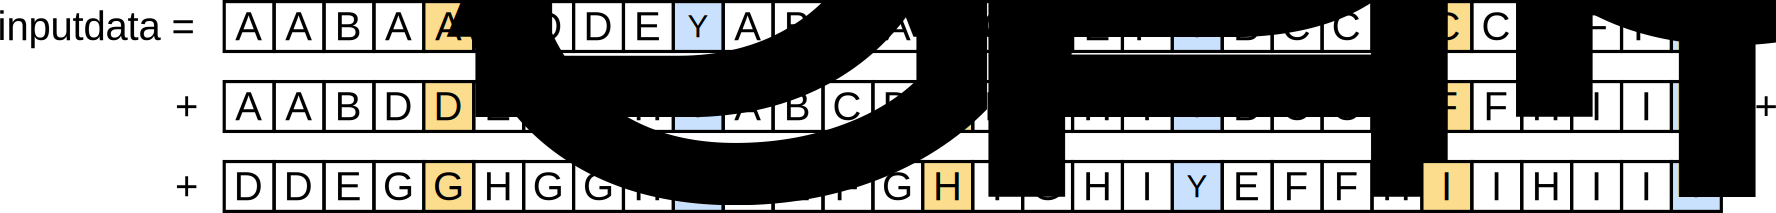
\includegraphics[width=0.75\textwidth]{fig/simdlayout-seq}
    }
    \vskip1\baselineskip
    \subfigure[Struktura dat pro vektorové zpracování]{
        \centering
        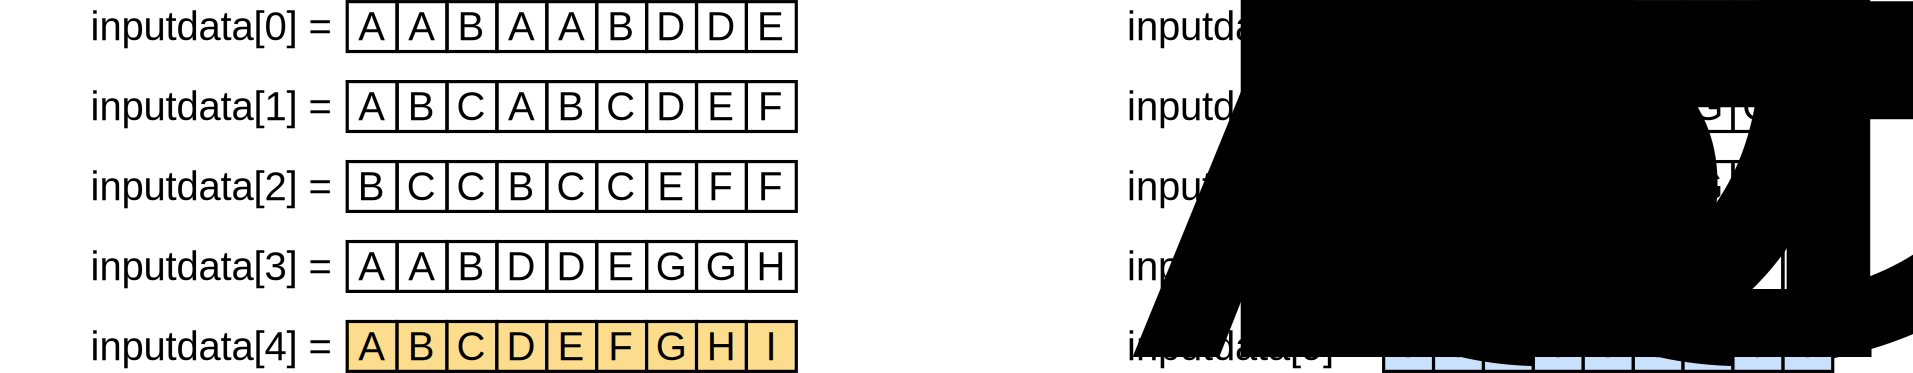
\includegraphics[width=0.75\textwidth]{fig/simdlayout-vect}
    }
    \caption{Uspořádání vstupních dat v~paměti pro sekvenční a vektorové zpracování. Žlutě je označen střed devítiokolí, modře požadovaný výstup filtru.}
    \label{obrDevitiokoli}
\end{figure}


\section{Sběr statistických dat}
\label{secImplExperimental}

Běh evoluce a její výsledky jsou pro pozdější statistické zpracování zaznamenávány do souborů. Každý typ výstupu obsluhuje samostatný modul, které se přihlašují k~odběru událostí~-- jde o~návrhový vzor \emph{pozorovatel} (\emph{observer}). Události vznikají v~hlavní smyčce evoluce a jsou následně předávány všem odběratelům, jak znázorňuje obrázek~\ref{obrLoggersHandling}.

\begin{figure}[b]
    \centering
    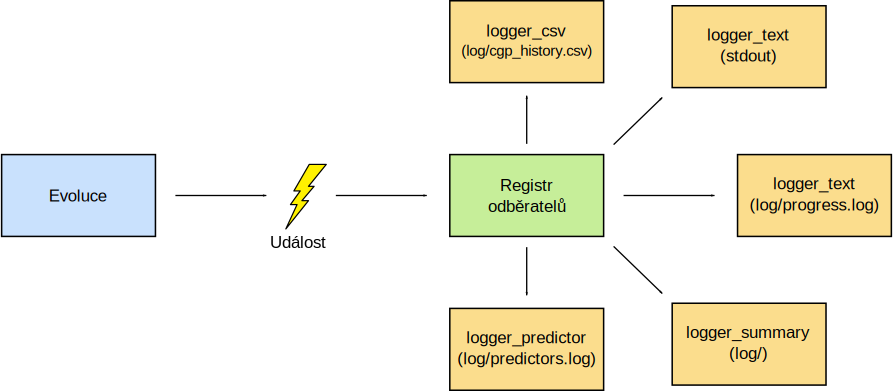
\includegraphics[width=0.75\textwidth]{fig/loggerevent}
    \caption{Způsob obsluhy událostí vzniklých během evoluce (např. nalezení lepšího kandidátního řešení) za účelem sběru statistických dat.}
    \label{obrLoggersHandling}
\end{figure}

Implementace jednotlivých obslužných modulů událostí je inspirovaná objektovým programováním. Základním datovým typem je struktura \texttt{struct logger\_base} (\uv{abstraktní třída}), která obsahuje položky pro ukazatele na obslužné funkce, konfiguraci programu a čas počátku evoluce. Prvním parametrem každé obslužné funkce je ukazatel na proměnnou tohoto typu (\uv{instanci třídy}), v~jejímž kontextu se má obsluha události provést. Pokud některý modul pro svůj běh potřebuje uchovávat další údaje (například jméno cílového souboru), může definovat vlastní datový typ (\uv{odvozenou třídu}), přičemž jeho první položka musí být typu \texttt{struct logger\_base}. Explicitním přetypováním lze s~takovou proměnnou pak pracovat stejně, jako by byla přímo typu \texttt{struct logger\_base}. Tímto se částečně simuluje dědičnost tříd a polymorfismus~-- při předávání události odběrateli není třeba znát jeho konkrétní datový typ. Všechny implementované datové typy jsou uvedeny na obrázku~\ref{obrLoggersTypes}.

\begin{figure}[htb]
    \centering
    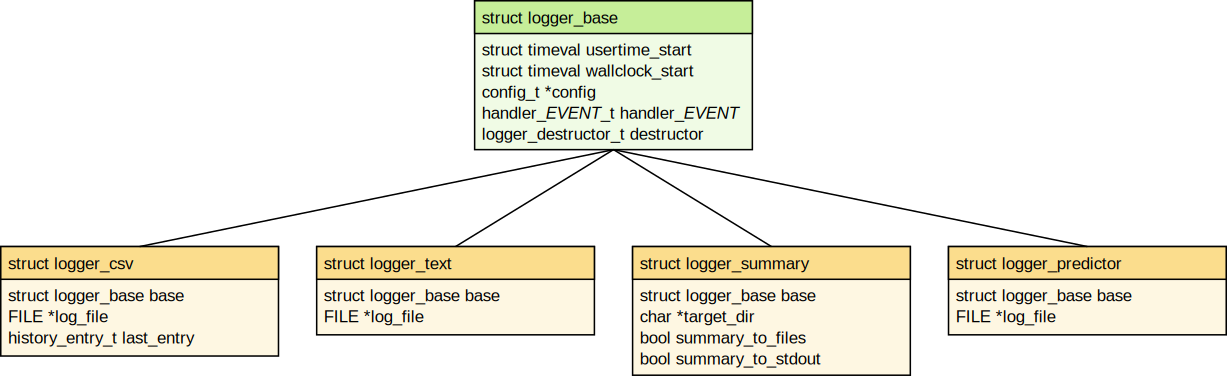
\includegraphics[width=\textwidth]{fig/loggertypes}
    \caption{Datové typy modulů obsluhující události a jejich hierarchie.}
    \label{obrLoggersTypes}
\end{figure}

Ve výchozím nastavení se k~obsluze událostí zaregistruje pouze jedna \uv{instance} typu \texttt{logger\_text}, který zapisuje na standardní výstup vybrané události v~čitelné podobě. Pokud se v~příkazové řádce uvede jméno cílové složky pro záznam evoluce, zaregistruje se druhá \uv{instance}, která bude totéž zapisovat do souboru. Také se zaregistrují \uv{objekty} typů \texttt{logger\_csv} a \texttt{logger\_summary}. První z~nich zapisuje průběh evoluce ve formátu CSV, který je pro další strojové zpracování vhodnější než textový výpis. Druhý zapíše do jednotlivých souborů nejlepší nalezený filtr a příslušný výstupní obrázek, celou konfiguraci programu a také soubor s~krátkým shrnutím výsledků. Nejlepší nalezený filtr je uložen do cílové složky v~jednoduchém textovém formátu, jako kód v~jazyce C a také v~grafické podobě (\emph{ASCII Art}) snadno srozumitelné pro uživatele. Dalším parametrem příkazové řádky lze zapnout ukládání všech použitých prediktorů do cílové složky, což zajišťuje \uv{instance} typu \texttt{logger\_predictor}.

V~budoucnu je možné poměrně snadno přidat další implementace obsluhy událostí. Nabízí se například vytvořit modul, který by informace o~průběhu evoluce zasílal grafickému uživatelskému rozhraní.

\section{Generování náhodných čísel}

Protože genetické algoritmy jsou ze své povahy stochastické, je potřeba v~implementaci použít nějaký zdroj náhodných nebo pseudonáhodných čísel. Nejjednodušší je použít funkci \texttt{rand} obsaženou ve standardní knihovně. Protože experimenty se budou spouštět dávkově, není vhodné pro inicializaci pseudonáhodné posloupnosti použít funkci \texttt{time}, která vrací datum a čas s~přesností na sekundy. Všechny běhy spuštěné ve stejné sekundě by pak byly inicializovány stejnou hodnotou a pracovaly se stejnou posloupností čísel.

Vhodnější je pro inicializaci použít funkci \texttt{gettimeofday}, která vrací aktuální čas od půlnoci s~přesností na mikrosekundy. Pravděpodobnost, že dva běhy použijí pro inicializaci totožnou hodnotu je pak velmi malá, přestože se čísla mohou každých 24 hodin opakovat.

%\section{Podpůrné nástroje}
%
%Kromě samotného evolučního návrhu obrazových filtrů je součástí implementace i několik pomocných nástrojů pro další zpracování výstupních dat.
%\todo{podpůrné nástroje - apply, predvis, predhist}


\section{Překlad programu}

Program je rozdělen do několika modulů. Jejich překlad a sestavení výsledného programu je definován v~Makefile a spouští se příkazem \texttt{make}. Je potřeba překladač GCC ve verzi alespoň 4.8, lépe ve verzi 4.9, která má dokonalejší podporu SIMD instrukcí, zejména umí využít všechny dostupné registry. Jednotlivé moduly programu se překládají samostatně do složky \texttt{build}. Při změnách ve zdrojovém kódu tak není nutné opakovaně překládat moduly, do kterých se nezasahovalo. Výstupem překladu je několik spustitelných souborů:

\begin{itemize}
    \item \texttt{coco}\footnote{Název \texttt{coco} je zkratka pro COlearning in COevolution.} -- hlavní program, samotný evoluční návrh obrazových filtrů,
    \item \texttt{coco\_apply} -- aplikace filtru uloženého v~souboru \texttt{*.chr} na libovolný obrázek,
    \item \texttt{coco\_predvis} -- vizualizace použitých prediktorů fitness,
    \item \texttt{coco\_predhist} -- tvorba histogramu pixelů používaných v~prediktorech fitness.
\end{itemize}

Jejich použití popisuje uživatelská příručka v~příloze~\ref{apxManual}.

\chapter{Experimentální vyhodnocení}
\label{chExperiments}

Tato kapitola popisuje provedené experimenty a parametry testovacího prostředí a také srovnání výsledků získaných navrženým algoritmem s~adaptivní velikostí prediktorů fitness, koevolucí s~prediktory pevné délky a také se standardním CGP bez koevoluce.

Všechny výpočty byly prováděny na superpočítači Anselm, který provozuje Národní superpočítačové centrum IT4Innovations. Skládá se celkem z~209 výpočetních uzlů, z~toho 180 obsahuje vždy dva osmijádrové procesory Intel Xeon E5-2665 (2,4 až 3,1\,GHz s~technologií Turbo Boost) a 64 GB operační paměti. Zbývající uzly mají po dvou procesorech Intel Xeon E5-2470 (2,3 až 3,1\,GHz s~technologií Turbo Boost) a alespoň 96 GB operační paměti \cite{AnselmSpecs}.

\section{Testovací problémy}

Pro srovnání navrženého algoritmu se standardním (ko)evolučním CGP byly vybrány tři úlohy z~oblasti zpracování obrazu.

V~prvním případě je cílem nalézt vhodný obrazový filtr pro rekonstrukci obrázků poškozených šumem typu sůl a pepř. U~tohoto šumu jsou poškozené pixely buď bílé nebo černé -- mají minimální nebo maximální možnou hodnotu. Příčinou mohou být vadné body ve snímači v~kameře, nefunkční paměťové buňky, k~poškození může dojít také během přenosu dat. Z~konvenčních filtrů je možné použít mediánový, během filtrování ale dochází ke ztrátě detailů a výsledky při vyšší intenzitě šumu nejsou uspokojivé. Druhým typem šumu použitém během experimentování je výstřelový šum. V~tomto případě mají poškozené pixely zcela náhodnou hodnotu. U~tohoto typu šumu lze také použít mediánový filtr, se stejnými omezeními. V~obou případech je šum charakterizován svou intenzitou -- poměrným počtem poškozených pixelů. Pro evoluci filtrů byl použit obrázek~\ref{obrTrenovaciLena}.

Poslední testovací úloha spočívá v~nalezení filtru, který provádí detekci hran v~obrazu. Výstupem detektoru je jednobitový černobílý obrázek, ve kterém jsou hrany označeny bílou barvou. Mezi konvenční filtry patří Sobelův nebo Cannyho detektor hran. V~tomto případě byly filtry trénovány na obrázku~\ref{obrTrenovaciPan}.

\begin{figure}[htb]
    \centering
    \subfigure[Šum sůl a pepř a výstřelový šum]{
        \hskip0.75cm
        \centering
            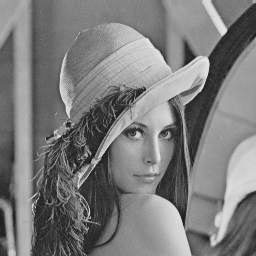
\includegraphics[width=0.3\textwidth]{fig/lena_gray_256.png}
        \label{obrTrenovaciLena}
        \hskip0.75cm
    }
    \subfigure[Detekce hran]{
        \hskip0.75cm
        \centering
            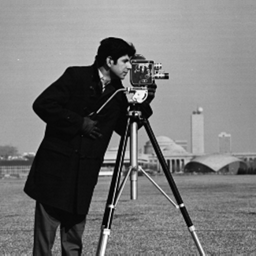
\includegraphics[width=0.3\textwidth]{fig/cameraman_256.png}
        \label{obrTrenovaciPan}
        \hskip0.75cm
    }
    \caption{Obrázky používané pro evoluci filtrů.}
    \label{obrTrenovaci}
\end{figure}

\section{Parametry evoluce}

Parametry CGP a koevoluce vychází z~článku \cite{SikuPPSN}. Kartézské genetické programování pracuje s~mřížkou o~8 sloupcích a 4 řádcích, $l$-back je roven jedné. Každý program má 9 primárních vstupů, na které jsou přiváděny devítiokolí pixelů trénovacího obrázku a jeden výstup, který určuje filtrovanou hodnotu pixelu uprostřed devítiokolí. V~populaci je celkem 8 jedinců, přičemž jeden z~nich se stává rodičem populace a potomci jsou od něj odvozeni mutací 1 až 5 genů. Průběh evoluce je podrobněji popsán v~kapitole~\ref{secCGP}.

Populace prediktorů fitness obsahuje 32 jedinců, kteří se vyvíjejí genetickým algoritmem popsaným v~kapitole~\ref{secGA}. Po ohodnocení jedinců v~populaci je tvořena nová třemi druhy jedinců. Jedna čtvrtina nové populace vznikne prostým zkopírováním nejlepších 8 jedinců z~předešlé generace. Druhá čtvrtina je vytvořena zcela náhodně, což vede na vyšší diverzitu jedinců a brání to degradaci populace. Zbylých 16 jedinců vznikne křížením a mutací. Rodiče těchto jedinců určuje turnaj, v~němž mezi sebou soupeří vždy dva náhodně zvolení jedinci. Jejich potomek pak vznikne jednobodovým křížením a následnou mutací až 5\,\% genů.

\section{Parametry souběžného učení}

V~této práci je představen modifikovaný algoritmus koevoluce s~prediktory fitness, kdy je navíc možná průběžně adaptovat velikost prediktorů na průběh evoluce fitness kandidátních kartézských programů. Tato nová část algoritmu vyžaduje několik nových parametrů, jejichž optimální hodnotu je třeba určit experimentálně. Tato část se popisuje, jakým způsobem různá nastavení těchto parametrů ovlivňují kvalitu nacházených obrazových filtrů a také celkovou rychlost programu.

\subsection{Nepřesnost predikce}

Ukázalo se, že pokud má prediktor dostatečnou délku, bývá hodnota predikované fitness velmi blízko hodnotě skutečné fitness. Avšak v~případě, že je prediktor již příliš krátký, může být predikovaná fitness i několikanásobně vyšší. Jako vhodná mez, kdy nepřesnost predikce již negativně ovlivňuje průběh evoluce obrazových filtrů, se ukázala hodnota $I_\mathit{threshold} = 1,2$. Po jejím překročení jsou prediktory skokově prodlouženy na dvojnásobek ($c_I = 2$).

\subsection{Změna velikosti prediktorů}

Pro každý z~parametrů byly testovány hodnoty z~intervalu $0,8$ až $1,1$ (s~krokem $0,01$), přičemž ostatní parametry měly fixní hodnoty. Počáteční velikost prediktoru byla nastavena na 50\,\% všech případů fitness. Evoluce byla ukončena po dosažení 30 tisíc generací CGP.

\subsubsection*{Při neměnné fitness filtrů}

Za stagnující vývoj je považován stav, kdy je absolutní hodnota rychlosti evoluce $|v|$ nižší než hodnota parametru $v_\mathit{zero}$, který byl ve všech případech nastaven na $0,001$. Velikost prediktorů se v~tomto případě upravuje pomocí koeficientu $c_0$. Pro každou testovanou hodnotu bylo spuštěno celkem 100 nezávislých běhů.

Jak je vidět na grafech~\ref{plotZerocoef-30kg}, hodnota parametru $c_0$ neovlivňuje kvalitu nalezených filtrů. Ukazuje se ale, že tento parametr určuje trend změny velikosti prediktorů a tím i dobu výpočtu. U~nižších hodnot velikost prediktoru v~průběhu evoluce klesá. S~rostoucí hodnotou má křivka průběhu velikosti prediktorů stále menší sklon a od hodnoty 0,94 velikost prediktorů už spíše roste. Pokud se hodnota parametru $c_0$ dále zvyšuje, tak se pouze urychluje konvergence velikosti k~maximální hodnotě.

\begin{figure}[tbp]
    \centering
    \subfigure[Kvalita nalezených filtrů]{
        \centering
           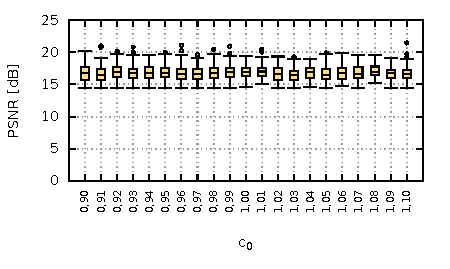
\includegraphics[width=0.95\textwidth]{fig/plot/tuning-zerocoef-30kg-psnr.pdf}
    }
    \subfigure[Doba běhu programu (součet všech vláken)]{
        \centering
            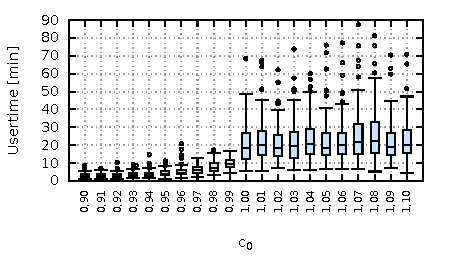
\includegraphics[width=0.95\textwidth]{fig/plot/tuning-zerocoef-30kg-utime.pdf}
    }
    \subfigure[Průběh velikosti prediktorů (průměr ze 100 běhů)]{
        \centering
            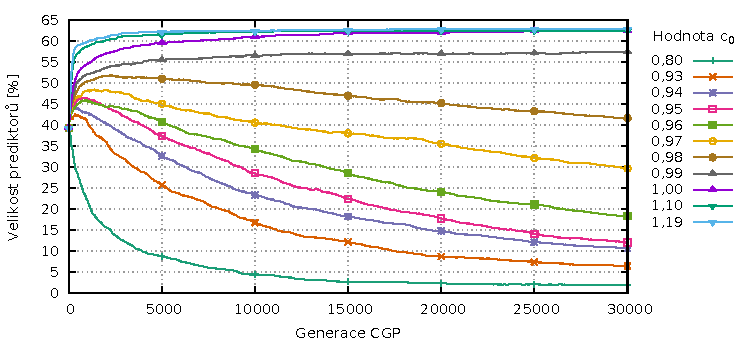
\includegraphics[width=0.95\textwidth]{fig/plot/tuning-zerocoef-30kg-predlen.pdf}
    }
    \caption{Vliv parametru $c_0$ (změna velikosti prediktoru při neměnné fitness filtrů)}
    \label{plotZerocoef-30kg}
\end{figure}

\subsubsection*{Při klesající fitness filtrů}

Druhé z~pravidel se aplikuje v~případě, že skutečná fitness nejlepšího jedince v~populaci filtrů klesá ($v < -v_\mathit{zero}$). Velikost prediktoru se pak upraví dle parametru $c_{-1}$. U~tohoto parametru byly testovány hodnoty $0,8$ až $1,1$, dosažené výsledky z~24 nezávislých běhů znázorňují grafy na obrázku~\ref{plotDecrcoef-30kg}. Tento parametr má větší vliv na kvalitu filtrů než parametr $c_0$, i když není úplně zřejmá vazba mezi hodnotou $c_{-1}$ a dosaženou kvalitou. Jako optimální se z~tohoto pohledu jeví hodnoty $0,96$ a $0,97$. Také lze pozorovat, že s~vyšší hodnotou roste i počet evaluací CGP a tím i doba běhu programu, i když ne tak razantně, jako v~případě parametru $c_0$. Zajímavá je hodnota $c_{-1} = 1,00$, kdy se velikost prediktoru nijak nemění -- v~tomto případě je algoritmus výrazně pomalejší než v~případě jiných okolních hodnot. Zřejmě je pro evoluci výhodnější změna velikosti prediktoru jakýmkoliv směrem (a tím i změna predikované fitness filtrů), než pokud k~žádné úpravě nedojde.

\begin{figure}[tbp]
    \centering
    \subfigure[Kvalita nalezených filtrů]{
        \centering
           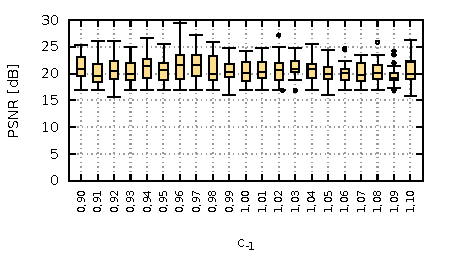
\includegraphics[width=0.95\textwidth]{fig/plot/tuning-decrcoef-30kg-psnr.pdf}
    }
    \vskip2\baselineskip
    \subfigure[Doba běhu programu (součet všech vláken)]{
        \centering
            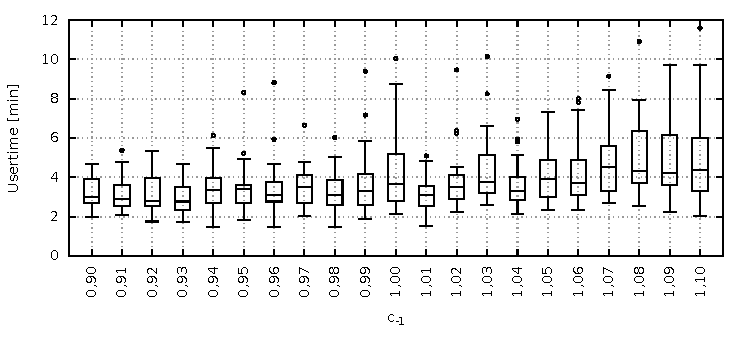
\includegraphics[width=0.95\textwidth]{fig/plot/tuning-decrcoef-30kg-utime.pdf}
    }
    \caption{Vliv parametru $c_{-1}$ (změna velikosti prediktoru při klesající fitness filtrů)}
    \label{plotDecrcoef-30kg}
\end{figure}

\subsection*{Při rostoucí fitness filtrů}

Pokud je rychlost $v$ vyšší než nula, rozlišuje se \uv{pomalý} a \uv{rychlý} nárůst fitness, čemuž odpovídají koeficienty $c_{+1}$ a $c_{+2}$. Jako práh byla zvolena hodnota $v_\mathit{slow} = 0,1$. Nejvhodnější hodnota obou parametrů byla hledána zvlášť, pro každé nastavení bylo spuštěno 100 běhů.

V~případě, že fitness filtrů roste pomaleji, uplatní se parametr $c_{+1}$. Jak je vidět na grafech na obrázku~\ref{plotSlowcoef-30kg}, nemá jeho hodnota znatelný vliv na kvalitu filtrů. Podobně jako u~jiných parametrů ovlivňující práci s~velikostí prediktorů, má vyšší hodnota za následek pomalejší běh programu, ale rozdíl není natolik výrazný. Také zde je při nastavení $c_{+1}$ potřebný čas vyšší, než u~okolních hodnot.

Také v~případě parametru $c_{+2}$ se ukazuje, že kvalita filtrů se příliš nemění, viz grafy na obrázku~\ref{plotFastcoef-30kg}. Při pohledu na čas běhu programu se zdá, že je výhodnější i v~tomto případě prediktory zkracovat. To je ale v~rozporu s~předpokladem (uvedeným v~části~\ref{secDesignAdaptation}), že pokud fitness filtrů roste, tak je vhodné prodlužovat prediktory a zpřesňovat predikovanou fitness. Ukazuje se, že je to způsobeno počáteční velikostí prediktorů (50\,\%), protože ta v~průběhu evoluce konverguje k~podstatně nižší hodnotě (jednotky procent), a proto je ve všech případech výhodnější zkracování. Pokud se počáteční velikost nastaví na 3\,\%, odpovídá chování předpokladům a vliv parametru $c_{+2}$ na čas běhu programu není tak výrazný, jak je vidět na grafu~\ref{plotFastcoef-30kg-utime-i3}.

\begin{figure}[p]
    \centering
    \subfigure[Kvalita nalezených filtrů]{
        \centering
           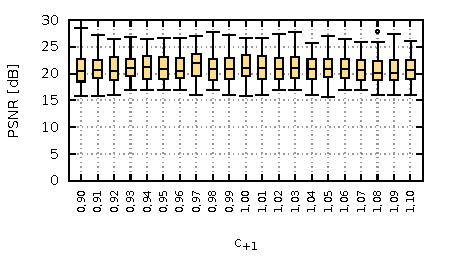
\includegraphics[width=0.95\textwidth]{fig/plot/tuning-slowcoef-30kg-psnr.pdf}
    }
    \vskip2\baselineskip
    \subfigure[Doba běhu programu (součet všech vláken)]{
        \centering
            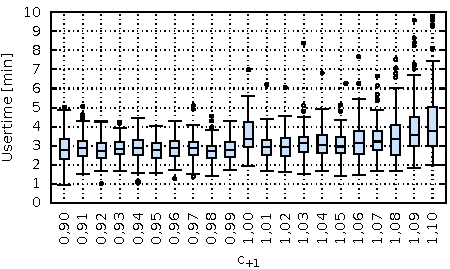
\includegraphics[width=0.95\textwidth]{fig/plot/tuning-slowcoef-30kg-utime.pdf}
    }
    \caption{Vliv parametru $c_{+1}$ (změna velikosti prediktoru při pomalu rostoucí fitness filtrů)}
    \label{plotSlowcoef-30kg}
\end{figure}

\begin{figure}[p]
    \centering
    \subfigure[Kvalita nalezených filtrů, počáteční velikost 50\,\%]{
        \centering
           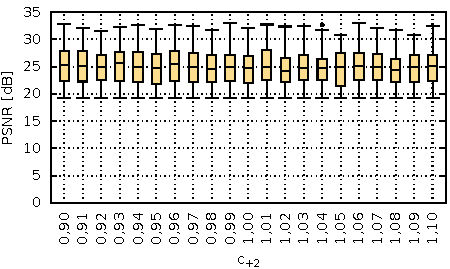
\includegraphics[width=0.95\textwidth]{fig/plot/tuning-fastcoef-i50-30kg-psnr.pdf}
    }
    \subfigure[Doba běhu programu (součet všech vláken), počáteční velikost 50\,\%]{
        \centering
            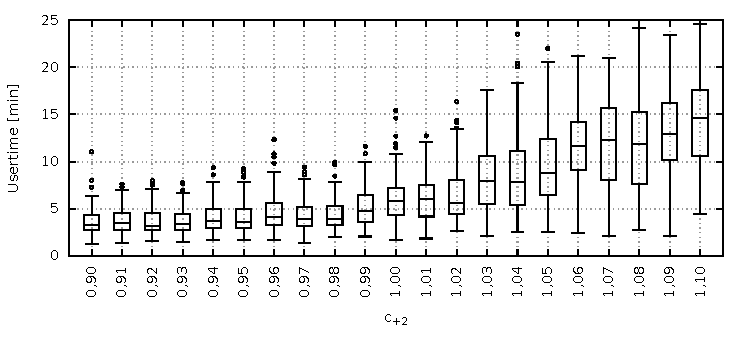
\includegraphics[width=0.95\textwidth]{fig/plot/tuning-fastcoef-i50-30kg-utime.pdf}
    }
    \subfigure[Doba běhu programu (součet všech vláken), počáteční velikost 3\,\%]{
        \centering
            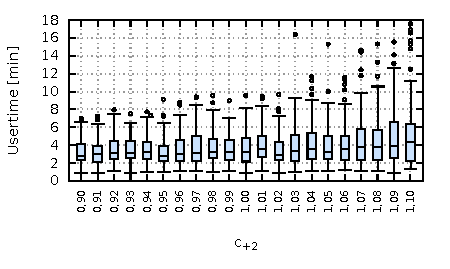
\includegraphics[width=0.95\textwidth]{fig/plot/tuning-fastcoef-i3-30kg-utime.pdf}
        \label{plotFastcoef-30kg-utime-i3}
    }
    \caption{Vliv parametru $c_{+2}$ (změna velikosti prediktoru při rychle rostoucí fitness filtrů)}
    \label{plotFastcoef-30kg}
\end{figure}


\subsection{Četnost změny velikosti prediktoru}

Jak bylo zmíněno v~kapitole~\ref{secDesignAdaptation}, ke změně velikosti prediktoru dochází při každé výměně rodiče v~populaci filtrů. Volitelným parametrem lze ale nastavit, aby ke změně velikosti došlo nejpozději po uběhnutí určitém počtu generací CGP od poslední změny. Testovány byly hodnoty 1~000, 2~500, 5~000 a 7~500 generací, přičemž evoluce byla ukončena po 30 tisících generacích. Po porovnání výsledků získaných ze sta nezávislých běhů se ukazuje, že tento parametr nemá příliš vliv ani na rychlost programu, ani na kvalitu filtrů.

\todo{prepocitat - pocital jsem s~january15, kde 1k vypadal nadejne (+1\,dB), ale u~november15 nedelal nic moc}

\subsection{Inicializace prediktorů}

Při tvorbě nových prediktorů fitness je nejjednodušší vytvořit jejich genom zcela náhodně. \todo{nevyhody?} Genom lze ale také inicializovat pomocí permutace všech možných hodnot.

Ukazuje se ovšem, že při inicializaci permutací, mají získané obrazové filtry v~průměru o~něco menší fitness. Zdá se, že větší náhodnost genů je pro evoluci výhodnější.

\todo{random, perm}

\subsection{Výpočet rychlosti evoluce}

\todo{last, avg7w, avg3, med3}

\subsection{Počáteční velikost prediktoru}

%Hlavním cílem této práce je nalézt algoritmus,

%Cílem tohoto experimentu je ověřit chování algoritmu při různé počáteční velikosti prediktoru -- ostatní parametry jsou ve všech případech stejné. V ideálním případě bude velikost prediktoru konvergovat pokaždé ke stejné hodnotě.

Pro ověření schopnosti adaptace velikosti prediktoru na řešený problém byla provedena řada výpočtů s~různou počáteční velikostí prediktoru. Jako testovací problém byl zvolen šum typu sůl a pepř o~intenzitě 5, 10, 15, 25 a 50 procent. Počáteční délka prediktoru byla 3\,\% a od 5 do 100\,\% případů fitness s~krokem po pěti procentech. Tato velikost určuje počet genů použitých pro tvorbu fenotypu prediktoru, fenotyp pak je o~něco kratší kvůli duplicitám v~genomu. Ve všech případech byla sledována průměrná velikost ze 100 nezávislých běhů.

Ukazuje se, že pokaždé velikost prediktoru konverguje ke stejné hodnotě, jak je vidět na grafech na obrázku~\ref{plotInitialSize-30kg}. Ta závisí na intenzitě šumu, při nejnižší intezitě 5\,\% je konečná velikost okolo 25\,\% celkového počtu pixelů, při nejvyšším 50\% šumu velikost konverguje ke 3 procentům. Také fitness nacházených filtrů je vždy přibližně stejná. Rychlost konvergence velikosti se liší podle typu šumu. U~5\,\% šumu už zhruba po šesti tisících generacích má prediktor přibližně 20\,\% případů fitness, zatímco v~případě 50\% šumu je potřeba asi 30 až 40 tisíc generací než velikost dosáhne zmíněná 3 procenta. Protože délka prediktoru má zásadní vliv na rychlost běhu programu, je výhodnější začínat s~menšími prediktory -- jako ideální se z~testovaných hodnot jeví počáteční velikost 3\,\% celkového počtu případů fitness.

% \begin{table}[htbp]
%     \renewcommand{\arraystretch}{1.2}
%     \centering
%     \begin{tabular}{|r|r|r|r|r|r|}
%         \hline
%         počáteční velikost & 5\,\% šum & 10\,\% šum & 15\,\% šum & 25\,\% šum & 50\,\% šum \\
%         \hline
%             3\,\%   & 20.6\,\% & 22.8\,\% & 9.5\,\%  & 7.0\,\% & 6.9\,\% \\
%             5\,\%   & 21.2\,\% & 17.4\,\% & 10.1\,\% & 2.7\,\% & 0.7\,\% \\
%             10\,\%  & 23.9\,\% & 19.0\,\% & 10.3\,\% & 3.7\,\% & 1.1\,\% \\
%             15\,\%  & 19.6\,\% & 16.8\,\% & 9.4\,\%  & 3.4\,\% & 1.4\,\% \\
%             20\,\%  & 20.7\,\% & 17.7\,\% & 7.9\,\%  & 3.4\,\% & 1.6\,\% \\
%             25\,\%  & 22.1\,\% & 19.0\,\% & 8.7\,\%  & 3.9\,\% & 2.0\,\% \\
%             30\,\%  & 22.6\,\% & 19.0\,\% & 8.0\,\%  & 3.6\,\% & 2.0\,\% \\
%             35\,\%  & 20.3\,\% & 18.2\,\% & 9.5\,\%  & 2.9\,\% & 0.5\,\% \\
%             40\,\%  & 20.9\,\% & 18.7\,\% & 9.7\,\%  & 4.4\,\% & 2.5\,\% \\
%             45\,\%  & 19.6\,\% & 21.1\,\% & 9.9\,\%  & 5.1\,\% & 2.7\,\% \\
%             50\,\%  & 21.8\,\% & 20.7\,\% & 8.7\,\%  & 4.4\,\% & 4.5\,\% \\
%             55\,\%  & 19.2\,\% & 22.3\,\% & 10.3\,\% & 4.1\,\% & 4.0\,\% \\
%             60\,\%  & 23.6\,\% & 18.6\,\% & 9.9\,\%  & 3.1\,\% & 0.6\,\% \\
%             65\,\%  & 20.8\,\% & 18.9\,\% & 10.3\,\% & 5.9\,\% & 5.4\,\% \\
%             70\,\%  & 24.4\,\% & 22.0\,\% & 8.6\,\%  & 5.7\,\% & 6.0\,\% \\
%             75\,\%  & 21.6\,\% & 20.3\,\% & 9.6\,\%  & 6.0\,\% & 4.4\,\% \\
%             80\,\%  & 21.5\,\% & 21.7\,\% & 10.4\,\% & 5.2\,\% & 6.7\,\% \\
%             85\,\%  & 20.0\,\% & 20.7\,\% & 8.4\,\%  & 9.1\,\% & 7.3\,\% \\
%             90\,\%  & 22.3\,\% & 24.7\,\% & 10.1\,\% & 6.6\,\% & 6.9\,\% \\
%             95\,\%  & 24.4\,\% & 22.7\,\% & 8.3\,\%  & 6.5\,\% & 5.1\,\% \\
%             100\,\% & 24.1\,\% & 26.1\,\% & 10.1\,\% & 6.6\,\% & 5.5\,\% \\
%         \hline
%     \end{tabular}

%     \caption{Průměrná velikost prediktoru (ze 100 běhů) po 30~000 generacích.}
%     \label{tabCGPFunctions}
% \end{table}


%\hline
%šum / generace & 10~000 & 30~000 & 100~000 \\
%\hline
%5\,\% & 13,6 -- 19,4\,\% & 19,2 -- 24,4\,\% & 24,9 -- 31,9\,\% \\
%\hline

\begin{figure}[htbp]
    \centering
    \subfigure[5\% šum typu sůl a pepř]{
        \centering
            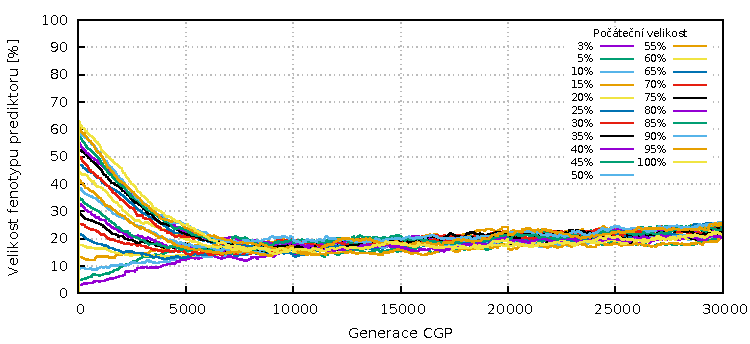
\includegraphics[width=0.95\textwidth]{fig/plot/initial-size/initial-size-5-30kg.pdf}
    }
    \subfigure[15\% šum typu sůl a pepř]{
        \centering
            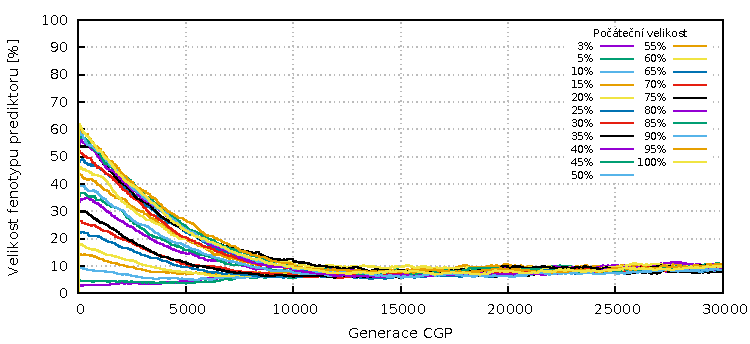
\includegraphics[width=0.95\textwidth]{fig/plot/initial-size/initial-size-15-30kg.pdf}
    }
    \subfigure[50\% šum typu sůl a pepř]{
        \centering
            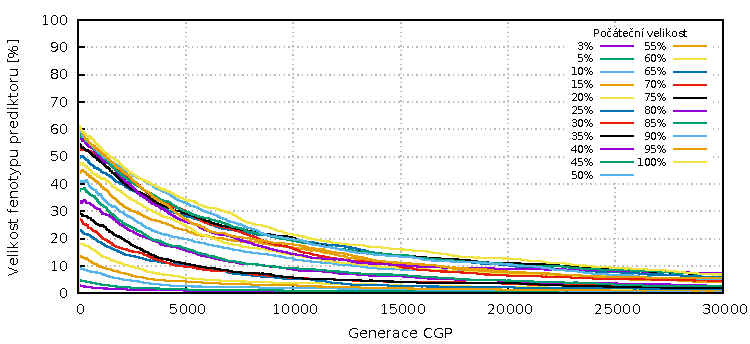
\includegraphics[width=0.95\textwidth]{fig/plot/initial-size/initial-size-50-30kg.pdf}
    }
    \caption{Vývoj velikosti prediktorů fitness při různé počáteční velikosti.}
    \label{plotInitialSize-30kg}
\end{figure}


\subsection{Zvolené hodnoty parametrů}

Na základě provedených experimentů byly pro souběžné učení zvoleny hodnoty parametrů, které jsou uvedeny v~tabulce~\ref{tabParams}.

\todo{by-max}

\begin{table}[h]
    \caption{Zvolené hodnoty parametrů souběžného učení}
    \renewcommand{\arraystretch}{1.2}
    \catcode`\-=12
    \centering
    \begin{tabular}{|l|l|c|l|l|}
        \cline{1-2}\cline{4-5}
        parametr & hodnota & & parametr & hodnota \\
        \cline{1-2}\cline{4-5}
        $I_\mathit{threshold}$ & 1,2   & & $v_\mathit{zero}$ & 0,001 \\
        $c_I$ & 2                      & & $v_\mathit{slow}$ & 0,1 \\
        $c_0$ & 0,90                   & & počáteční velikost prediktorů & 3\,\% \\
        $c_{-1}$ & 0,96                & & inicializace prediktorů & zcela náhodně \\
        $c_{+1}$ & 1,07                & & změna velikosti & jen při změně rodiče \\
        $c_{+2}$ & 1                   & & &\\
        \cline{1-2}\cline{4-5}
    \end{tabular}
    \label{tabParams}
\end{table}

% \begin{itemize}
%     \item $I_\mathit{threshold} = 1,2$,
%     \item $c_I = 2$,
%     \item $c_0 = 0,93$,
%     \item $c_{-1} = 0,96$,
%     \item $c_{+1} = 1,07$,
%     \item $c_{+2} = 1$,
%     \item $v_\mathit{zero} = 0.001$,
%     \item $v_\mathit{slow} = 0.1$,
%     \item počáteční velikost prediktoru: 3\,\% počtu případů fitness,
%     \item inicializace prediktorů zcela náhodně.
% \end{itemize}


\section{Chování souběžného učení}
\todo{chovani soubezneho uceni - vzit si jeden beh, vysvetlit ruzne pocatecni velikosti}
\todo{Statistika pravidel: jak často které}
\todo{Rychlost mezi populacemi}

\todo{vizualizace prediktorů - červeně i histogramem, také pro částečně poškozenou lenu}

\section{Srovnání souběžného učení, koevoluce a CGP}

\fixme{Cílem experimentů bylo srovnání navrženého algoritmu CGP s~adaptivními prediktory fitness ($\mathit{FP_{ADAPT}}$) s~koevolučním CGP s~prediktory pevné délky ($\mathit{FP_{FIX}}$) a s~CGP bez koevoluce ($\mathit{CGP_{STD}}$) s~ohledem na kvalitu nalezených obrazových filtrů a na délku běhu evoluce. Experimenty byly provedeny na obrázcích se šumem o~intenzitě 10 až 80\,\% s~krokem po 10\,\%.

Jak je vidět na příkladu 10\% výstřelového šumu na obrázku~\ref{fig:ImpulseBoxplot}, je kvalita filtrů nalezená pomocí $\mathit{FP_{ADAPT}}$ srovnatelná s~filtry získanými $\mathit{CGP_{STD}}$ a $\mathit{FP_{FIX}}$ s~pre\-dik\-tory o~velikosti 10\,\% a více. Co se týče potřebného času, je v~tomto případě $\mathit{FP_{ADAPT}}$ v~průměru 6,26krát rychlejší než $\mathit{CGP_{STD}}$. Také je srovnatelně rychlý jako při použití $\mathit{FP_{FIX}}$ s~3--5\% pre\-dik\-to\-rem, kdy ale mají výsledné filtry nižší kvalitu než u~$\mathit{FP_{ADAPT}}$.

Podobné výsledky byly dosaženy i pro jiné in\-ten\-zity šumu. Konkrétní hodnoty jsou uvedeny v~tabulce~\ref{table:results}. Ve všech případech je kvalita filtrů získaných pomocí $\mathit{FP_{ADAPT}}$ srovnatelná při kratší nebo přinejhorším podobné době běhu. V~průměru bylo dosaženo 8,39násobného zrychlení oproti $\mathit{CGP_{STD}}$.}

\subsection{Šum sůl a pepř}

% \afterpage{%
%     \clearpage% Flush earlier floats (otherwise order might not be correct)
%     \thispagestyle{empty}% empty page style (?)
%     \begin{landscape}% Landscape page
%         \centering % Center table
%         \begin{tabular}{|l|*{27}{l|}}
%             \hline
%              velikost prediktoru & \multicolumn{3}{c|}{CGP} & \multicolumn{3}{c|}{0,5\,\%} & \multicolumn{3}{c|}{1\,\%} & \multicolumn{3}{c|}{5\,\%} & \multicolumn{3}{c|}{10\,\%} & \multicolumn{3}{c|}{15\,\%} & \multicolumn{3}{c|}{20\,\%} & \multicolumn{3}{c|}{25\,\%} & \multicolumn{3}{c|}{Souběžné učení} \\
%             \hline

%             intenzita šumu & min. & max. & med. & min. & max. & med. & min. & max. & med. & min. & max. & med. & min. & max. & med. & min. & max. & med. & min. & max. & med. & min. & max. & med. & min. & max. & med. \\
%             \hline

%             5\,\% & 23,5 & 41,4 & 34,5 & 34,9 \\

%             \end{tabular}
%         \captionof{table}{Table caption}% Add 'table' caption
%     \end{landscape}
%     \clearpage% Flush page
% }

\subsection{Výstřelový šum}

\subsection{Detektor hran}



\chapter{Závěr}
\label{chConclusions}

Tento semestrální projekt se zabývá problematikou evolučních algoritmů, evolučního návrhu obrazových filtrů a vztahem mezi učením a evolucí. Následně je navržen systém pro tvorbu obrazových filtrů využívající souběžné učení v~koevoluci s~prediktory fitness. Použití souběžného učení by mělo pomoci překonat některé nedostatky koevolučního algoritmu, zejména nutnost experimentálně nalézt nejvhodnější velikost prediktoru fitness.

% Kapitola~\ref{chEA} postupně představuje principy evolučních algoritmů, genetického algoritmu, kartézského genetického programování, použití koevoluce a v~závěru se zabývá souběžným učením a plasticitou fitness. Následující kapitola~\ref{chDesign} je věnována návrhu systému pro tvorbu obrazových filtrů s~použitím souběžného učení.

V~navazující diplomové práci bude navržený systém implementován a následně otestován. Experimenty budou zaměřeny především na kvalitu výsledných filtrů a čas běhu programu. Výsledky dosažené při použití souběžného učení budou porovnány s~implementací koevoluce používající prediktory fitness pevné délky a také se variantou, kdy je prediktor fitness generován programem vyvíjeným pomocí kartézského genetického programování.

Tato práce byla publikována na studentské konferenci Excel@FIT 2015, kde byla vybrána k~ústní prezentaci jako jeden z~12 nejzajímavějších příspěvků.
